\section{Introduction}


A Josephson junction is a quantum mechanical device composed of two superconducting electrodes separated by a weak link \cite{Barone:1982}.
For currents lower than a critical value $I_C$, coupled electrons (Cooper pairs) can cross the weak link without a potential difference (dc Josephson effect).
%the device behaves as an uninterrupted superconductor and coupled electrons (Cooper pairs) can cross the weak link without any voltage drop.
When the current is increased above $I_C$, single electrons originated by the breakup of Cooper pairs begin to traverse the weak link. The potential difference $V$ between the two superconducting films becomes $\neq 0$ and a state is reached where the junction behaves as a resistance.

In modern Josephson junctions the weak link is usually a thin insulating tunnel barrier (SIS junction) \cite{Gurvitch:1983}, a normal metal film (SNS junction) \cite{Benz:1995} or a physical nanoconstriction (ScS junction) \cite{Cybart:2015, DeLeo:2016}. Josephson junctions have found wide usage in several research fields, for example as building blocks for RSFQ digital electronics  or quantum computers \cite{Likharev:1991}, or as radiation detectors and very sensitive magnetometers (SQUIDs) \cite{Maggi:2006b, Troeman:2007, Granata:2015}.
But the most successful application of Josephson junctions is surely in voltage metrology.
A microwave radiation of frequency $f$ can phase lock the junction oscillations, producing the so-called Shapiro-steps, i.e., current steps at the quantized voltages $V_n$, 

\begin{equation}
	V_n = n \frac{h}{2 e} f, \quad n = 1, 2, ...
\label{eq:voltage_steps}
\end{equation}

where $h$ and $e$ are the Plank constant and electron charge, respectively. The ac Josephson effect is at the basis of the current quantum voltage standard.
%that from 1987 replaced the previous voltage standard based on Weston cells.

Besides its practical applications, the Josephson junction is important from a physical point of view because it has been the first device showing a quantum mechanical effect on a macroscopic scale.

%% However, only in the second half of the 80’s, the development of the reliable Nb/Al-AlO,/Nb fabrication process made it possible to reach quantized voltages of $1$ and $10$~V, suitable for direct dc voltage calibration. These devices were based on large series arrays of thousands of SIS Josephson junctions (here SIS stands for superconductor-insulator-superconductor, where Nb is the superconducting film and the Al0, layer is the insulating tunneling barrier of the junction).

%% The Josephson voltage standard at the $1$ and $10$~V levels that were the state-of-the-art implementation at the time and were deployed only in very few labs wordwide, required a very careful engineering of the microwave distribution lines within the many arms in which the Josephson arrays were divided. 

An important research topic at the beginning of the '90s was related to finding ways to increase the amplitude of the current steps induced by the microwave radiation (rf-induced steps). In fact, the stability of the lock between the phase of the junction and the applied microwave radiation -- and therefore its insensitivity to noise events which might switch the junction from one quantized voltage to another, a crucial problem for voltage standard applications -- is strongly dependent on the amplitude of the steps \cite{Kautz:1987}.

To increase the amplitude of the current steps, a non-sinusoidal microwave radiation may be used.
%when two phased microwaves of frequencies $f$ and $2 f$ are added together, the rf-induced current steps can have normalized amplitudes larger than those predicted for a standard sinusoidal radiation 
In 1990 Monaco showed that, in the limit of a voltage-biased Josephson junction, adding together two phased microwaves of frequency $f$ and $2 f$ produces rf-induced current steps whose amplitudes are larger than those observed with a sinusoidal radiation \cite{Monaco:1990}.

Experiments on the so-called ``biharmonic drive'' readily confirmed these conclusions, albeit with some limitations due to the fact that the junctions could not realistically be considered as voltage biased \cite{Andreone:1991, Andreone:1992}.

%Experiments on the so-called ``biharmonic drive'' readily confirmed, at least in part, these conclusions. The differences were due to the fact that the junctions could not realistically be considered as voltage biased \cite{Andreone:1991, Andreone:1992}.

Extending further the idea, Monaco showed that, still in the limit of voltage bias, if the microwave radiation is composed of a train of delta functions, the rf-induced current steps could become as large as the critical current $I_C$.

However, a voltage bias configuration does not properly model a real Josephson junction, which  should usually be considered as current biased.
Also, a pulse train composed of delta functions is only a theoretical approximation and cannot be reproduced in actual experiments.
This led to the idea to investigate what happened to a current-biased Josephson junction irradiated by a more realistic pulsed microwave signal \cite{Maggi:1996, Maggi:1997}. 
The reproduction of this investigation is the object of the present work.



\section{Computational context}
\label{computational-context}

A first attempt to solve this problem was made using an electronic analog simulator of a Josephson junction \cite {Henry:1981}, that could compute the relation between the applied current and the voltage ($I-V$ characteristic) of a current-biased junction, in the framework of the Stewart-McCumber RSJ junction model \cite{McCumber:1968, Stewart:1974}.
The analog simulator was fast and simple to use, and could produce in just a few minutes beautiful plots of the $I-V$ characteristics of the junction as a function of the simulated microwave signal on a \href{http://www.hpmuseum.net/display_item.php?hw=74}{Hewlett Packard 7475A}2 pen plotter.
%\footnote{A brief description of the \href{http://www.hpmuseum.net/display_item.php?hw=74}{HP 7475A pen plotter} can be found on the HP Computer Museum.}
\footnote{Unfortunately, after 25 years and two relocations, I could not manage to find photographs of the simulator nor the original HP 7475A plots.} 

%The real problem with this approach was that, 
However, even if the electronic simulation was extremely fast, the analysis of the results required to measure by hand the amplitude of the rf-induced steps visible on each $I-V$ characteristic, a long and error-prone work.

Therefore, I decided to write a Fortran program to solve numerically the nonlinear second-order differential equation that models the Josephson junction \cite{McCumber:1968, Stewart:1974}. 
The idea was to calculate the $I-V$ characteristics of the junction as a function of the amplitude of the microwave signal, $\alpha_\mathrm{rf}$, for a given set of parameters characterizing the junction and the microwave, considering the three different cases of standard sinusoidal drive, biharmonic drive and pulsed drive.

To ease comparison of the results, normalized units were used throughout the calculations. The normalized junction voltage was $\eta$ and the normalized current $\alpha$.
The main parameters of the simulation were: hysteresis parameter $\beta$, microwave frequency $\Omega$, amplitude of the microwave signal $\alpha_\mathrm{rf}$, width of the pulsed signal $\rho$. 
For a given set of junction parameters, usually $100$ different $I-V$ characteristics for increasing or decreasing values of $\alpha_\mathrm{rf}$ were calculated.

The first versions of the Fortran program were compiled under DOS 6.22 with \href{https://winworldpc.com/product/microsoft-fortran/5x}{Microsoft Fortran 5.1} and run on what was then a state-of-the-art PC, probably a Compaq Deskpro 486 with a math coprocessor, shared among several users of the lab.

After a few attempts, the limitations of a PC for such a task soon become evident.
A new simulation started automatically each evening and took the entire night to complete. Regrettably, people still using the PC late in the evening often stopped the background process or simply shut the machine down without checking if there was another job running. 
At the end, I could run a full simulation only every two or three days.

After a few weeks of these mostly unsuccessful attempts, a colleague of another research group proposed me to use four DEC workstations running ULTRIX for my own simulations.\footnote{The now defunct \href{https://en.wikipedia.org/wiki/Digital_Equipment_Corporation}{Digital Equipment Corporation} (DEC) was one of the leading computer companies of the time.}
The machines were heavily used by his group during working hours, but sat mostly idle overnight. 
If I could manage to finish my runs before the start of the new work day, I was allowed to use this idle time for my own simulations.
The colleague gave me a quick crash course on Unix and I was ready to go.
%\footnote{I should still have my notes somewhere.}

Porting my Fortran program from Microsoft Fortran 5.1 to ULTRIX was a breeze, and I quickly learnt how to use FTP to transfer the input configuration files and the output data files containing the results of the simulation back and forth from the DEC workstations to my Compaq 386 notebook, that was also my desktop computer.
%\footnote{I was one of the \emph{happy few} to have a personal computer sitting on my own desk.}

Now each day I had four different sets of data files coming from the DEC workstations. Three of them were obtained by irradiating the junction with a pulsed drive with decreasing values of $\rho$, while keeping constant $\beta$ and $\Omega$.
The fourth simulation was made by irradiating the junction with a sinusoidal signal, while keeping everything else equal. This last simulation was used as a reference, to compare the results obtained with a standard sinusoidal radiation with those obtained with progressively shorter pulses.
Each night I changed the values of $\beta$ or $\Omega$, to study the effect of these parameters on the behavior of the junction.

Again, the real problem was how to analyze all this data. A manual analysis like that needed with the electronic simulator was out of consideration. 
I decided to try the recently released Microsoft Visual Basic 1.0 for Windows, writing another program that calculated the size of all the rf-induced steps visible on the $I-V$ characteristics of the nightly simulations, as a function of $\alpha_\mathrm{rf}$.
%Everything worked flawlessly.
%Now I could transfer by FTP the files containing the nightly results from the DEC workstations to my desktop computer and 
Running the Visual Basic program on each set of data files produced a summary file that contained the size of the calculated current steps.

The results of months of calculations were summarized in a paper published in the Journal of Applied Physics \cite{Maggi:1996}.



\section{Digging into code} \label{sec:digging-into-code}

%Finding the original sources of this project was easy and complex at the same time.
I like organisation, and I try keep all my past projects on my main workstation. 
Thus, finding the original source and data files of this project was only a question of locating the directory where the project was stored.
Problems started to arise when I looked at the different files. The whole project was scattered into several directories, each containing many files with widely different names and dates. At first, trying to find an order in that chaos seemed impossible.

Normally I would have found all information needed in many notebooks full of detailed handwritten notes.
% Normally it would have been only a question of recovering all needed information from my handwritten notebooks for this project
Unfortunately, a couple of years ago most of my work notebooks were damaged by a water leak in the basement, and could not be recovered. So the only option left was to check the files one by one. 
It is a great luck that modern operating system greatly ease the burden of dealing with data files; macOS in particular offers Quick Look, an exceptional tool to quickly browse through hundreds of files at the touch of the spacebar.

%%some with  misleading names such as \texttt{old} or \texttt{obsolete}, which one was older? (turns out that \texttt{obsolete} is \emph{older} that \texttt{old}).

After a thorough inspection of the whole project I recalled that:
(1) my first attempts with the numerical simulations tried to use the more accurate McDonald-Johnson junction model \cite{McDonald:1976}, I later switched to the simplified Stewart-McCumber RSJ model because it was much faster and efficient in calculating the junction behavior \cite{McCumber:1968, Stewart:1974};
(2) file names attempted to reflect what the programs actually did:\footnote{At least within the limits of DOS 8+3 naming scheme, only 8 characters for the file name and 3 characters for the extension.} 
in the same directory I could have a file ending with a "t" that provided a textual output and another file ending with a "g" that gave a graphical output.
These files differed only for a couple of \texttt{DEFINES}s, that instructed the compiler to choose the sections of the code that provided the textual or graphical output interface.
This multiplication of source files might seem senseless today, when comfortable graphical interfaces, ultra-fast text editors with support of regular expressions and version control tools allow to change a file in just a few seconds, but at that time it was probably the fastest, albeit very inefficient, way of working with source code;
(3) the header of all source files contained detailed notes about the type of program, the compiler, the type of output, and what probably mattered more, the dates of first and last revision of the source file, easying much the analysis of the different versions of the Fortran programs (Fig.~\ref{fig:source-header}); 
(4) the initial versions of the Fortran programs were monolithic, a single source file contained the whole code, consisting in about 1.000 lines of Fortran. Only at a later time, better computing practices led me to divide the monolithic code into multiple source files, compiled and linked together with a \texttt{Makefile}.
%(I will not delve into it here, as it a different paper).

%===============================================================================
\begin{figure}[tb]
	\centering
	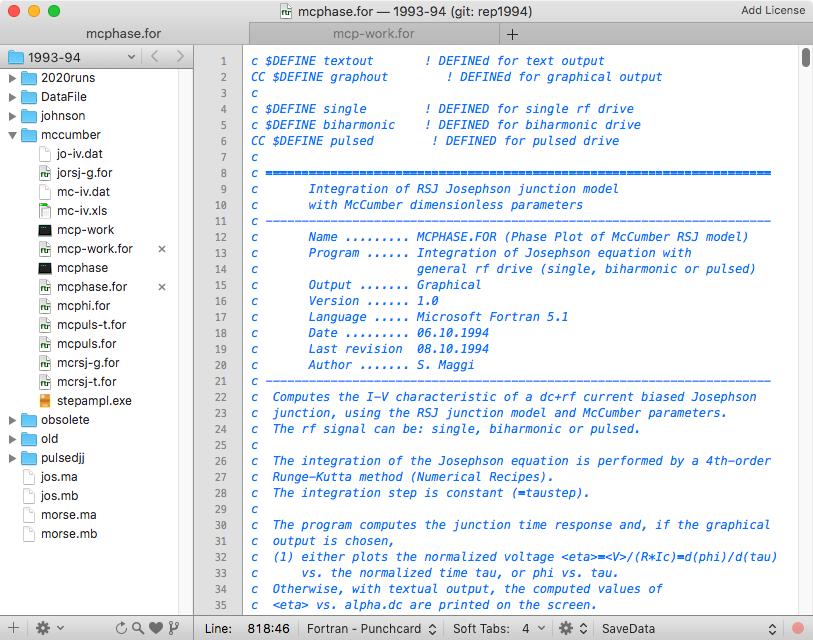
\includegraphics[width=0.75\textwidth]{source-header.png}
	\caption{Header of one of the Fortran source files. The left sidebar shows the directory structure of the project.}
	\label{fig:source-header}
\end{figure}
%===============================================================================


Another invaluable tool to analyze the different versions of the source files was \href{http://meldmerge.org/}{Meld}, an open source application available for all major operating systems that can perform a two- and even a three-way comparison of files and directories.
Using Meld I quickly realized that the two main source files were \texttt{mcphase.for} and \texttt{mcp-work.for}, both located in the \texttt{mccumber/} directory  (Fig.~\ref{fig:meld-comparison}).

%%===============================================================================
%\begin{figure}[bt]
%	\centering
%	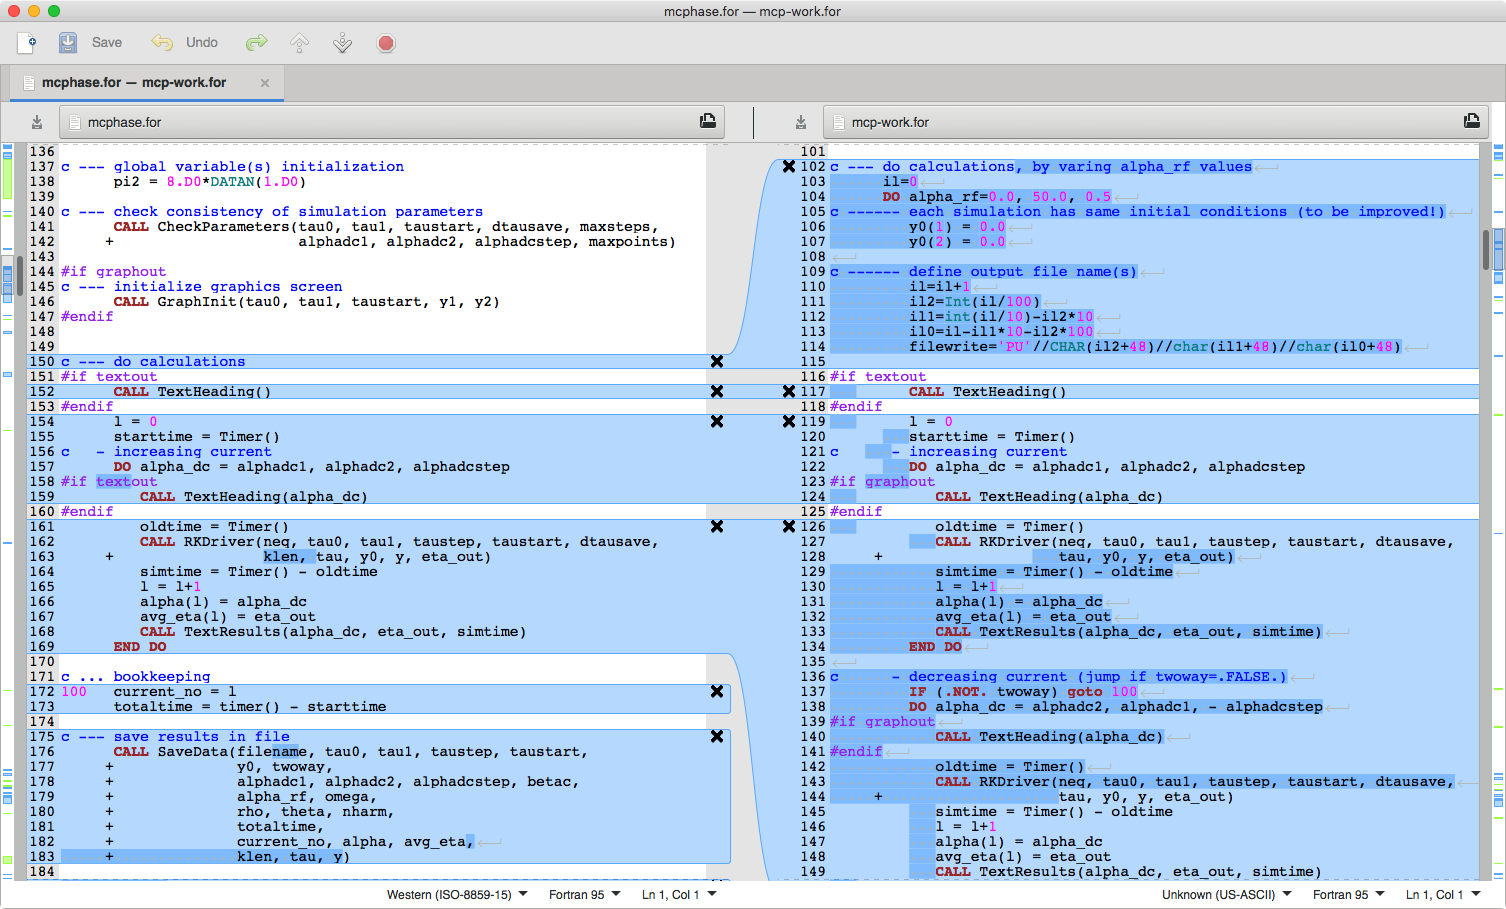
\includegraphics[width = 0.75 \textwidth]{meld-comparison.png}
%	\caption{Comparison with Meld of the main calculation loop of \texttt{mcphase.for} and \texttt{mcp-work.for}.}
%	\label{fig:meld-comparison}
%\end{figure}
%%===============================================================================


The first program, \texttt{mcphase.for}, simulated the behavior of the junction for a single value of $\alpha_\mathrm{rf}$, read from the input configuration file \texttt{iv.dat}, and saved the $I - V$ characteristic of the junction and its phase portrait (i.e., the relation between the phase and its time derivative, the latter being proportional to the junction voltage $V$) in the output file \texttt{iv.out}.

Multiple calculations with several different value of $\alpha_\mathrm{rf}$ could be performed by using a  DOS batch file that basically choose one by one the configuration files containing the desired values of $\alpha_\mathrm{rf}$, renamed them to \texttt{iv.dat}, run \texttt{mcphase} and at the end renamed the file containing the results, \texttt{iv.out}, using a consistent naming scheme.
%for each value of $\alpha_\mathrm{rf}$, copied a \texttt{.dat} input file containing the proper set of simulation parameters into a file with a standard name, \texttt{iv.dat}, run the simulation and at the end renamed the output file containing the results of the simulation, \texttt{iv.out} so that it has the same basename of the original \texttt{.dat} input file.
I don't recall why I choose this approach, but it was clearly very inefficient, as it required to prepare each day a long series of configuration files that differed only by the value of $\alpha_\mathrm{rf}$, and to update accordingly the DOS batch file that controlled the night calculations (Fig.~\ref{fig:batch-file}).

%%===============================================================================
%\begin{figure}[tbh]
%	\centering
%	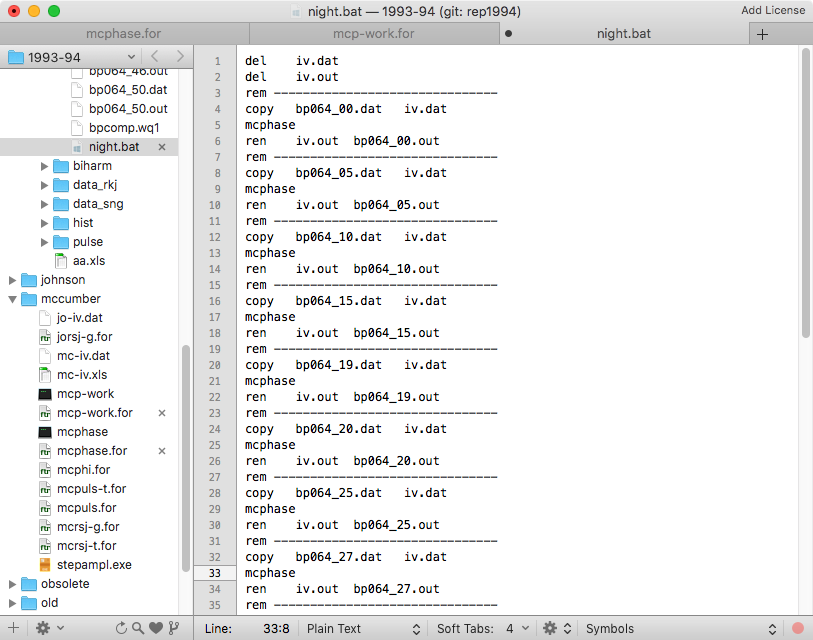
\includegraphics[width = 0.75 \textwidth]{batch-file.png}
%	\caption{DOS batch file used by \texttt{mcphase.for} to perform multiple simulations with different values of $\alpha_\mathrm{rf}$.}
%	\label{fig:batch-file}
%\end{figure}
%%===============================================================================


The second program, \texttt{mcp-work.for} was an improved version that could cycle across a  set of several values of $\alpha_\mathrm{rf}$, producing a different output file for each value of $\alpha_\mathrm{rf}$. To simplify the later automatic analysis, it left out the phase portrait.

Clearly this was the program ported to the DEC workstations. 
Unfortunately, I could not find the actual source file used on these machines, probably because I worked directly on the workstations and never thought to copy back these files to my PCs.
Luckily, Fortran is a very stable language and making \texttt{mcp-work.for} work on a modern machine was very easy.

As for the Microsoft Visual Basic 1.0 code, I found only two versions of the programs and the differences between them were minimal. Since both programs gave exactly the same results, I decided to stick with the version that had a still working pre-compiled binary.



\section{Porting Microsoft Fortran to modern Unix}

Porting \texttt{mcp-work.for} to the XXI century so that it could be compiled with the modern open source and multiplatform \texttt{gfortran} Fortran compiler was very easy, thanks to the stability of the language across different versions and platforms. Only a few minor tweaks to the source code were needed.

All work has been done on macOS, which is essentially BSD Unix with a more appealing graphical interface, but could be easily repeated on any modern Unix-like operating system such as Linux, and probably even on Windows, with the support of either the \href{https://docs.microsoft.com/en-us/windows/wsl/}{Windows Subsystem for Linux} (for Windows 10) or of \href{http://www.cygwin.org/}{Cygwin} (for earlier versions of the operating system).



\subsection{Preprocessor directives}

For reasons that go beyond my understanding Microsoft Fortran 5.1 did not use standard preprocessor directives, such as those supported by \texttt{cpp} or \texttt{fpp}, \cite{Boyanski:1992} but used a a slightly different proprietary syntax (Fig.~\ref{fig:preprocessor}). 
To support \texttt{cpp}, all was needed was to comment out all the \texttt{\$DEFINE} directives in the header section and to replace the Microsoft Fortran 5.1 \texttt{DEFINE} blocks with standard \texttt{cpp} blocks throughout the code (Fig.~\ref{fig:preprocessor}). 

The right compilation directives are chosen now at compile-time. For example, the following command
\footnote{The \texttt{\$} symbol prepended to this and all following terminal commands represents the prompt of the command interpreter and is not part of the command.}

%
% %===============================================================================
% \lstset{
%     language = C,
%     basicstyle = \tiny\bfseries\ttfamily,
%     tabsize = 4,
%     frame = lines,
%     framesep = 1em,
%     framexleftmargin = 1em,
%     backgroundcolor = \color{ultralightgray},
%     keywordstyle = \color{darkred}\bfseries,
%     morekeywords = {$DEFINE, $if, $endif, defined},
%     deletekeywords = {for}
% }
% %===============================================================================
% \begin{figure}[b]
% \centering
%
% \begin{minipage}{0.48\textwidth}
% \textbf{(a)}
% \begin{lstlisting}
% $DEFINE textout            ! DEFINEd for text output
% c $DEFINE graphout        ! DEFINEd for graphical output
%
% c $DEFINE single        ! DEFINED for single rf drive
% c $DEFINE biharmonic    ! DEFINED for biharmonic drive
% $DEFINE pulsed            ! DEFINED for pulsed drive
%
% $if defined (graphout)
%     ...
% $endif
% ...
% ...
% $if defined (textout)
%     ...
% $endif
% ...
% $if defined (pulsed)
%     ...
% $endif
% \end{lstlisting}
% \end{minipage}
% %
% \hfill
% %
% \begin{minipage}{0.48\textwidth}
% \textbf{(b)}
% \begin{lstlisting}
% CC $DEFINE textout        ! DEFINEd for text output
% c $DEFINE graphout        ! DEFINEd for graphical output
%
% c $DEFINE single        ! DEFINED for single rf drive
% c $DEFINE biharmonic    ! DEFINED for biharmonic drive
% CC $DEFINE pulsed        ! DEFINED for pulsed drive
%
% #if graphout
%     ...
% #endif
% ...
% ...
% #if textout
%     ...
% #endif
% ...
% #if pulsed
%     ...
% #endif
% \end{lstlisting}
% \end{minipage}
%
% \caption{Preprocessor directives in (a) Microsoft Fortran 5.1, (b) modern \texttt{cpp} preprocessor.}
% \label{fig:preprocessor}
% \end{figure}
% %===============================================================================
%


%===============================================================================
\lstset{
    language = bash,
    basicstyle = \small\bfseries\ttfamily,
    tabsize = 4,
    frame = none,
    framesep = 2em,
    framexleftmargin = 1em,
    backgroundcolor = \color{ultralightgray},
    keywordstyle = \color{darkred}\bfseries,
    morekeywords = {gfortran},
    deletekeywords = {for}
}
%===============================================================================
\begin{lstlisting}
$ gfortran -cpp -Dtextout -Dsingle -o mcp-work mcp-work.for
\end{lstlisting}
%===============================================================================

runs the \texttt{cpp} preprocessor before the gfortran compiler, selecting only the sections of the code that produce a textual output (\texttt{-Dtextout}) and perform the calculations with the sinusoidal drive (\texttt{-Dsingle}).



\subsection{Filenames}

Compilers based on Fortran 77, such as Microsoft Fortran 5.1, did not support dynamic memory allocation at runtime and required programmers to use fixed-length arrays and strings. Strings were used rather sparingly in Fortran code, so that was not a big deal. With an exception. 
My code defined the basename of all files as the 50-byte long character variable \texttt{filename},
%
%%===============================================================================
%\lstset{
%    language = Fortran,
%    tabsize = 6,
%    frame = none,
%    framesep = 2em,
%    framexleftmargin = 1em,
%    backgroundcolor = \color{ultralightgray},
%}
%%===============================================================================
%\begin{lstlisting}
%	CHARACTER*50   filename
%\end{lstlisting}
%%===============================================================================
%
attaching a proper extension to the input configuration file containing the simulation parameters and to the output data files with the results of the calculations.

Under DOS that was not a problem, as DOS truncates file names to only 8 characters plus 3 characters for the extension, and excess characters were simply ignored. But under Unix file names have no real limitations,\footnote{To be precise, Unix allows 255 characters for the filename and 4096 characters for the path.} and having all these 50 character-long filenames, mostly composed by blank characters, was ugly and complicated file management, in particular when using the command line interface.
The solution was simple, as Fortran now has the \texttt{TRIM} function that removes all trailing blanks from a string. 
Whenever a file is opened for reading or for writing, \texttt{TRIM()} is applied on-the-fly to the \texttt{filename} variable,

%===============================================================================
\begin{lstlisting}
	OPEN (UNIT = 10, FILE = TRIM(filename)//'.dat', STATUS = 'OLD')
\end{lstlisting}
%===============================================================================

thus removing all extra blanks from the name of the file.



\subsection{Edit descriptors}

Microsoft Fortran 5.1 used the non-standard backslash (textsf{\textbackslash{}}) edit descriptor to prevent the addition of a line break at the end of a \texttt{WRITE} instruction.
%\footnote{http://userweb.eng.gla.ac.uk/peter.smart/com/981124.htm}
Modern Fortran compilers do not support this edit descriptor and return an error. This problem is avoided by removing the backslash edit descriptor from all \texttt{WRITE} instructions that include it.



\subsection{Date and time}

Microsoft Fortran 5.1 had two separate intrinsic subroutines to return the current date and time.
In particular, \lstinline[columns=fixed]{CALL GETDAT(iyr, imon, iday)}, saved the date in the two-byte integer variables \texttt{iyr}, \texttt{imon} and \texttt{iday}, while \lstinline[columns=fixed]{CALL GETTIM(ihr, imin, imin, i100th)} did the same for the current time, saving the return values in the integer variables \texttt{ihr}, \texttt{imin}, \texttt{imin} and \texttt{i100th}. The meaning of each returned variable should be self-explanatory.

Modern Fortran supports the single subroutine \lstinline[columns=fixed]{CALL DATE_AND_TIME(DATE, TIME, ZONE, VALUES)}, where all arguments are optional and can be specified by their dummy names (i.e., how Fortran calls the keyword arguments of a function call). 
In particular, \texttt{DATE}, \texttt{TIME} and \texttt{ZONE} are character variables, while \texttt{VALUES} is a one-dimensional array of 8 integers, where \texttt{VALUES(1:3)} corresponds to the year, month and day of the month, \texttt{VALUES(4)} is the time difference (in minutes) with UTC, and \texttt{VALUES(5:8)} are the hour, minute, second and milliseconds, respectively.

To minimize changes to the original source code, the original calls to the \lstinline[columns=fixed]{GETDAT} and \lstinline[columns=fixed]{GETTIM} subroutines, were translated to a single call to \lstinline[columns=fixed]{DATE_AND_TIME}, assigning the elements of the returned array of \texttt{VALUES} to integer variables named as in the original code (Fig.~\ref{fig:date-time}).


%%===============================================================================
%\begin{lstlisting}
%	INTEGER*2      iyr, imon, iday
%	INTEGER*2      ihr, imin, isec, dummy
%	...
%	CALL GETDAT(iyr, imon, iday)
%	CALL GETTIM(ihr, imin, isec, dummy)
%\end{lstlisting}
%%===============================================================================


%%===============================================================================
%\begin{lstlisting}
%	character*8    date
%	character*10   time
%	character*5    zone
%	integer        values(8)
%	...
%	call date_and_time(date, time, zone, values)
%
%	iyr  = values(1)
%	imon = values(2)
%	iday = values(3)
%	ihr  = values(5)
%	imin = values(6)
%	isec = values(7)
%\end{lstlisting}
%%===============================================================================



\subsection{Compilation with gfortran}
\label{compilation-with-gfortran}

%All these fixes were enough to compile correctly \texttt{mcphase.for} with gfortran.
%As for \texttt{mcp-work.for}, basically it required the same corrections, with one rather strange addition.

As noted above, \texttt{mcp-work.for} calculates the $I - V$ characteristics of the simulated junction for several different values of $\alpha_\mathrm{rf}$, producing one output file for each $I - V$ curve. The section of the code that defined the names of the output files was quite convoluted,

%===============================================================================
\lstset{
    language = Fortran,
    tabsize = 6,
    frame = none,
    framesep = 2em,
    framexleftmargin = 1em,
    backgroundcolor = \color{ultralightgray},
	keywordstyle = \color{darkred}\bfseries,
	morekeywords = {},
	deletekeywords = {file name}
}
%===============================================================================
\begin{lstlisting}
      il=0
      DO alpha_rf=0.0, 50.0, 0.5
      ...
c ------ define output file name(s)
         il=il+1
         il2=INT(il/100)
         il1=INT(il/10)-il2*10
         il0=il-il1*10-il2*100
         filewrite='PU'//CHAR(il2+47)//CHAR(il1+47)//CHAR(il0+47)
      ...
      END DO        ! repeat alpha_rf DO cycle

\end{lstlisting}
%===============================================================================

and used the integer variable \texttt{il} to count the cycle number, while the three integers \texttt{il2}, \texttt{il1} and \texttt{il0} contained the hundreds, tens and units digits of \texttt{il}, respectively. 
The \texttt{CHAR} function converts these integers to the corresponding \texttt{ASCII} characters, where \texttt{ASCII} code 48 corresponds to the \texttt{0} symbol and \texttt{ASCII} code 57 corresponds to \texttt{9}.
The name of the output file defined in the variable \texttt{filewrite} was built by concatenating with the \texttt(//) operator a trailing constant string to the three \texttt{ASCII} characters (\texttt{'PU'} in the example above).

I have no idea why I decided to build the name the output files in such a complex way, while it would have been much simpler to use the value of $\alpha_\mathrm{rf}$ to name each output file.
In any case, it did not work under gfortran and prevented proper compilation of the code. 

After some inspection and testing, it was apparent that the source of the problem lied in the number \texttt{47} added to three integer variables before converting them to \texttt{ASCII} characters, that should be replaced by \texttt{48}. 
The line defining the \texttt{filewrite} variable thus becomes, %\lstinline[columns=fixed]{filewrite='PU'//CHAR(il2+48)//char(il1+48)//char(il0+48)}.

%===============================================================================
\begin{lstlisting}
      ...
      DO alpha_rf=0.0, 50.0, 0.5
      ...
c ------ define output file name(s)
         ...
         filewrite='PU'//CHAR(il2+48)//CHAR(il1+48)//CHAR(il0+48)
      ...
      END DO        ! repeat alpha_rf DO cycle
\end{lstlisting}
%===============================================================================

With this change \texttt{mcp-work.for} could compile flawlessly under gfortran.
What is really puzzling is how the original line could work in Microsoft Fortran 5.1.
%Microsoft Fortran required to add a \texttt{47} instead of \texttt{48} to convert a integer to the correct \texttt{ASCII} character.



\section{Visual Basic code}
\label{visual-basic-code}

No attempt was made to make the original Visual Basic 1.0 code run a modern computer. Visual Basic is a dead language and long since has been replaced by Visual Basic .NET, which shares only the name with its forefather. From the beginning, the only viable option to run a Visual Basic 1.0 program today was to rebuild the original development environment in an emulator.

I preferred to use the \href{https://www.parallels.com/}{Parallels Desktop} emulator for macOS, but the open source multiplatform \href{https://www.virtualbox.org/}{VirtualBox emulator} should work equally well.

I created a new empty virtual machine with minimal \emph{hardware} requirements and installed in sequence DOS 6.22, Windows 3.11 and Visual Basic 1.0 (Fig.~\ref{fig:windows-311}).
[++ While I was at it, and although I had already reproduced the Fortran part of the project, I also decided to install Microsoft Fortran 5.1 for DOS, to try to recreate as much as possible the original work environment. ++]

All software packages were downloaded from the \href{https://winworldpc.com}{WinWorld web site}, an invaluable resource for recovering old software packages. 
Even after so many years, the legitimacy of installing proprietary software in an emulator, might be questionable. But at the time I had regular licenses for all the above mentioned software and I guess to be at least morally authorized to continue to use those packages.

The packages were originally distributed on several floppy disks, which had to be swapped whenever the installer required a new disk. 
The installation of these software packages in an emulator is close to how it was done back then.
The only difference is that today the floppy disks are replaced by virtual file images and "swapping" disks is not done mechanically but requires to select a menu option in the emulator.

At the end of the installation process, the Windows 3.11 appeared as in (Fig.~\ref{fig:windows-311}).
%, in all its full $640 \times 480$ pixels glory.
The default $640 \times 480$ pixel screen resolution of Windows 3.11 was woefully meager by today's standards.
But, as I used the virtual environment almost exclusively to run the Visual Basic program, I didn't bother to install the drivers that could increase the screen resolution to a more comfortable $800 \times 600$ or $1024 \times 768$ pixel resolution.


%===============================================================================
\begin{figure}[t]
	\centering
	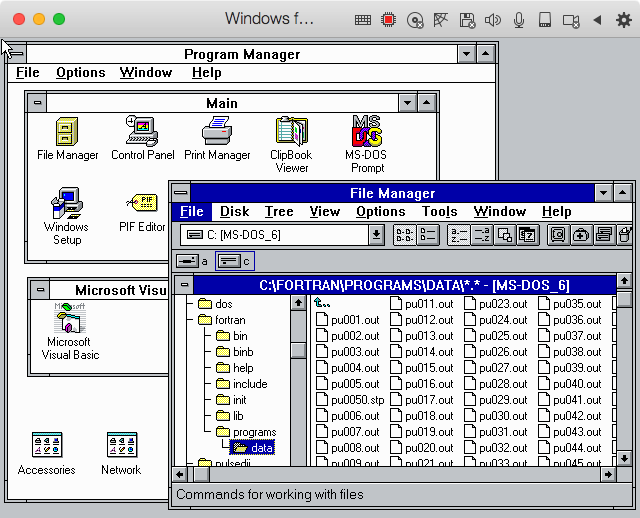
\includegraphics[width=0.75\textwidth]{windows-311.png}
	\caption{The Windows 3.11 desktop as shown in the Parallels emulator.}
	\label{fig:windows-311}
\end{figure}
%===============================================================================



Using the emulator required to transfer the source and binary Visual Basic files to the emulated DOS/Windows system.
It is surely possible to make the emulated Windows 3.11 communicate with the host operating system through the network. But I found much easier to use again a virtual floppy disk to transfer all needed files from macOS to Windows 3.11 (and viceversa).
%, mounted alternatively (end exclusively) on macOS or on Windows 3.11, 

A new empty virtual floppy disk \texttt{data.img} can be easily created with the command-line utility \texttt{dd} available on macOS or Linux, 
% \lstinline[columns=fixed]{dd if=/dev/zero of=data.img bs=1440k count=1}.

%%===============================================================================
%\lstset{
%    language = bash,
%    basicstyle = \small\bfseries\ttfamily,
%    tabsize = 4,
%    frame = none,
%    framesep = 2em,
%    framexleftmargin = 1em,
%    backgroundcolor = \color{ultralightgray},
%    keywordstyle = \color{darkred}\bfseries,
%%    morekeywords = {dd, if, of, bs, count},
%    morekeywords = {dd},
%    deletekeywords = {for}
%}
%%===============================================================================
%\begin{lstlisting}
%dd if=/dev/zero of=data.img bs=1440k count=1
%\end{lstlisting}
%%===============================================================================


After creation, the virtual floppy disk must be mounted in the emulator and formatted under DOS or Windows 3.11 in the original MS-DOS FAT file system.

[++ The same virtual floppy disk was used to copy the source code of \texttt{mcphase.for} and \texttt{mcp-work.for} and the \texttt{mc-iv.dat} configuration file to the virtual machine. ++]
%[++, transferring them to the Microsoft Fortran 5.1 standard project directories.++]

%[++ how did I find where these dirs were located??? ++]
%
%[++ The same was done for the Visual Basic project and the precompiled binary, creating a new directory in the virtual machine to host these files. ++]

This step completed the preparation of the development environment, now it was time to test how all this behaved.



\section{Running the programs}

%Running \texttt{mcphase.for} is easy. In summary, all I had to do was to compile \texttt{mcphase.for} with the right directives, switch to the \texttt{2020runs/} directory and run the \texttt{mcphase} executable from there, as summarized below,
%
%%===============================================================================
%\lstset{
%    language = bash,
%    basicstyle = \small\bfseries\ttfamily,
%    tabsize = 4,
%    frame = none,
%    framesep = 2em,
%    framexleftmargin = 1em,
%    backgroundcolor = \color{ultralightgray},
%    keywordstyle = \color{darkred}\bfseries,
%    alsoletter=-,
%    morekeywords = {gfortran},
%    deletekeywords = {for}
%}
%%===============================================================================
%\begin{lstlisting}
%$ gfortran -cpp -Dtextout -Dsingle -o mcphase mcphase.for
%$ cd ../2020runs/
%$ ../mccumber/mcp-work
%\end{lstlisting}
%%===============================================================================
%
%obtaining a file \texttt{mc-iv.out} that contains the $I - V$ characteristic and the phase portrait (the relation between the phase and its time derivative, the latter being proportional to the junction voltage $V$) of the junction for the set of parameters defined in \texttt{mc-iv.dat}. 
%The calculation takes only a couple of seconds to complete on a recent computer, and without microwave radiation ($\alpha_\mathrm{rf} = 0$), produces the well-known non-hysteretic $I - V$ characteristic of the RSJ model (Fig.~\ref{fig:iv-single}a), while for non-zero values of $\alpha_\mathrm{rf}$ the staircase-like structure of the rf-induced current steps appear on the $I - V$ curves (Fig.~\ref{fig:iv-single}b and Fig.~\ref{fig:iv-single}c).
%
%%===============================================================================
%\begin{figure}[bh]
%{
%	\fboxsep=0pt
%	\mbox{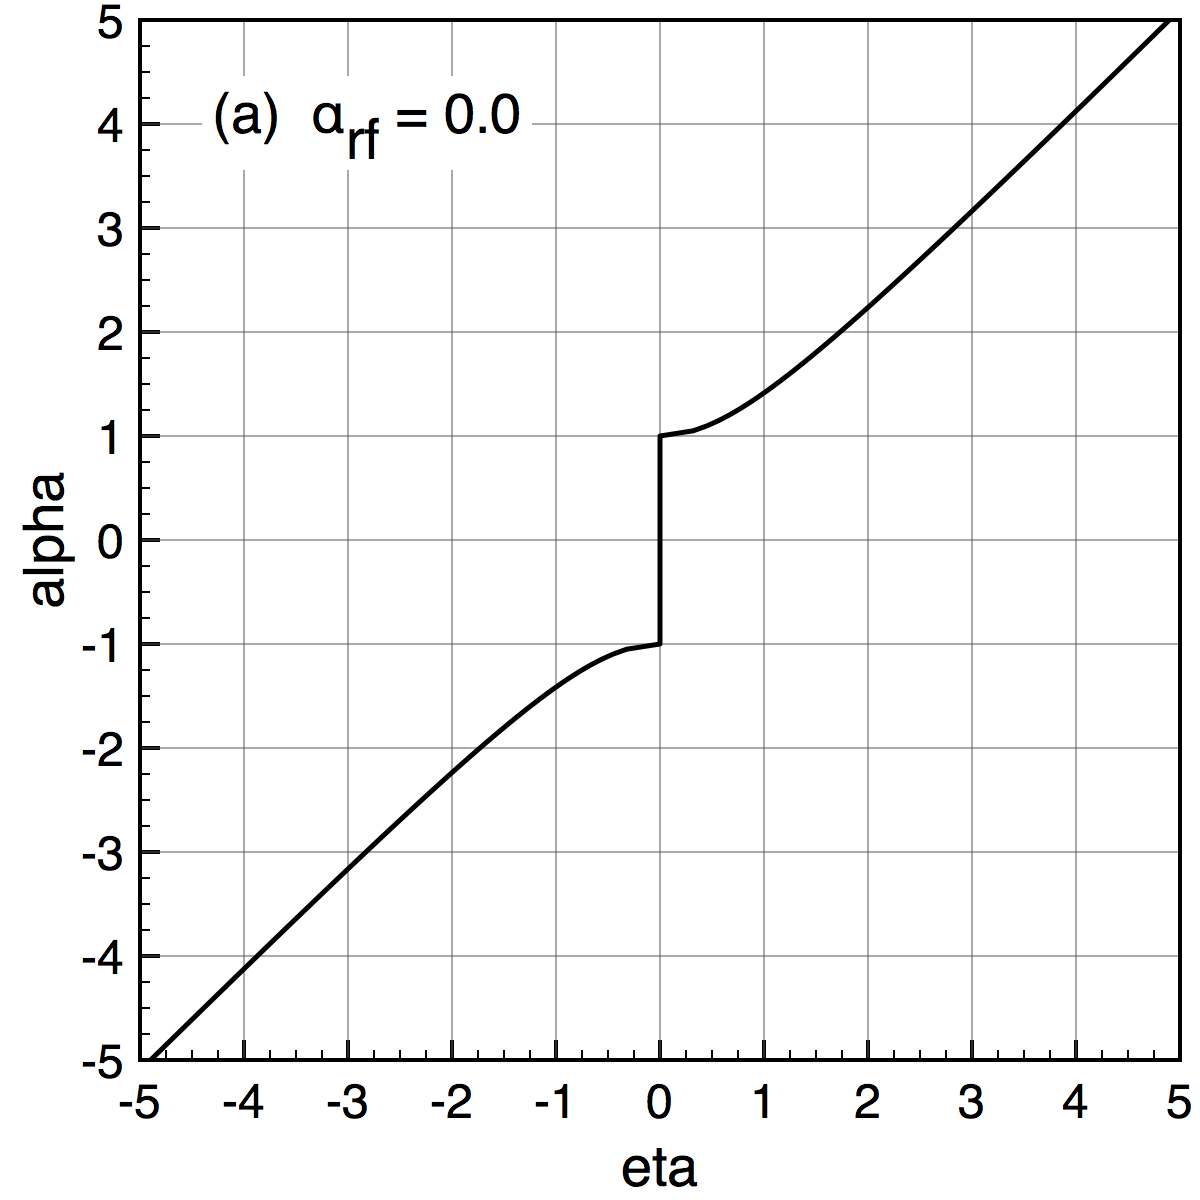
\includegraphics[width=0.325\textwidth]{iv-single-alpharf0.png}}
%	\hfill
%	\mbox{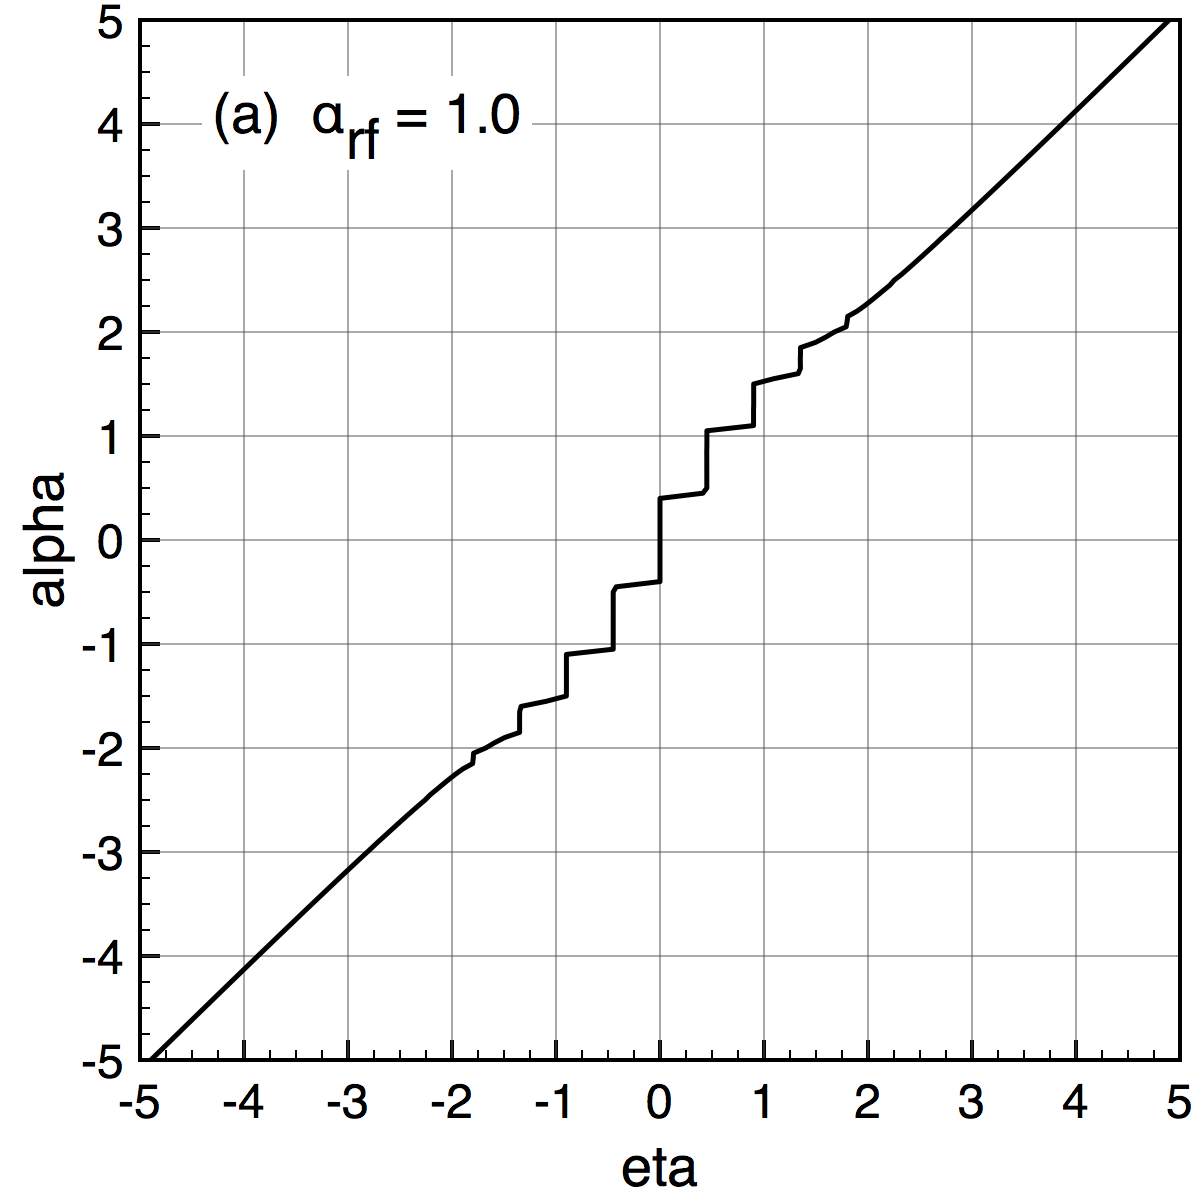
\includegraphics[width=0.325\textwidth]{iv-single-alpharf1.png}}
%	\hfill
%	\mbox{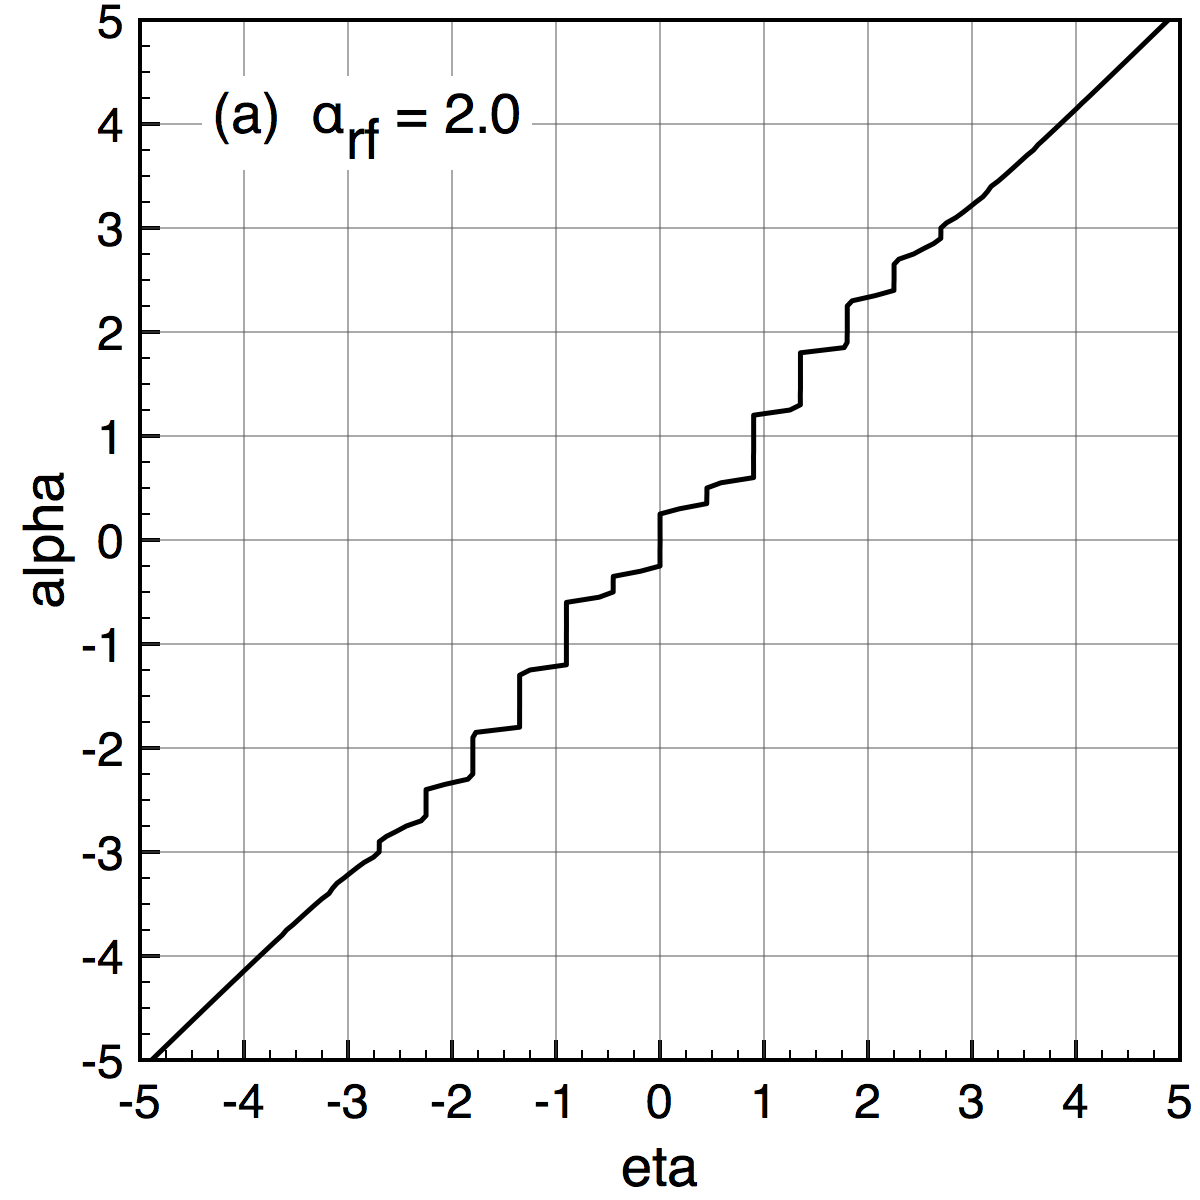
\includegraphics[width=0.325\textwidth]{iv-single-alpharf2.png}}
%}
%	\caption{$I - V$ characteristics of a junction with $\beta_c = 0.01$, driven by a sinusoidal rf bias of frequency $\Omega = 0.45$ and (a) $\alpha_\mathrm{rf} = 0.0$, (b) $\alpha_\mathrm{rf} = 1.0$ and (c) $\alpha_\mathrm{rf} = 2.0$. The rf-induced current steps are clearly visible when $\alpha_\mathrm{rf} > 0$. Here $\eta$ and $\alpha$ are the junction normalized voltage and current, respectively.}
%	\label{fig:iv-single}
%\end{figure}
%%===============================================================================
%
%
%To simulate a pulsed rf bias, it is sufficient to compile \texttt{mcphase.for} with the \texttt{-Dpulsed} directive and rerun the simulation (Fig.~\ref{fig:iv-pulsed}). 
%The $I - V$ characteristic without the rf bias is identical to that calculated with the sinusoidal signal (Fig.~\ref{fig:iv-pulsed}a), while the current steps induced by the pulsed drive are fewer and nearly as wide as the critical current for $\alpha_\mathrm{rf} = 0.0$ (compare Figs.~\ref{fig:iv-pulsed}a and \ref{fig:iv-pulsed}c).
%
%%%===============================================================================
%%\begin{lstlisting}
%%$ gfortran -cpp -Dtextout Dpulsed -o mcphase mcphase.for
%%$ cd ../2020runs/
%%$ ../mccumber/mcphase
%%\end{lstlisting}
%%%===============================================================================
%
%%===============================================================================
%\begin{figure}[bh]
%{
%	\fboxsep=0pt
%	\mbox{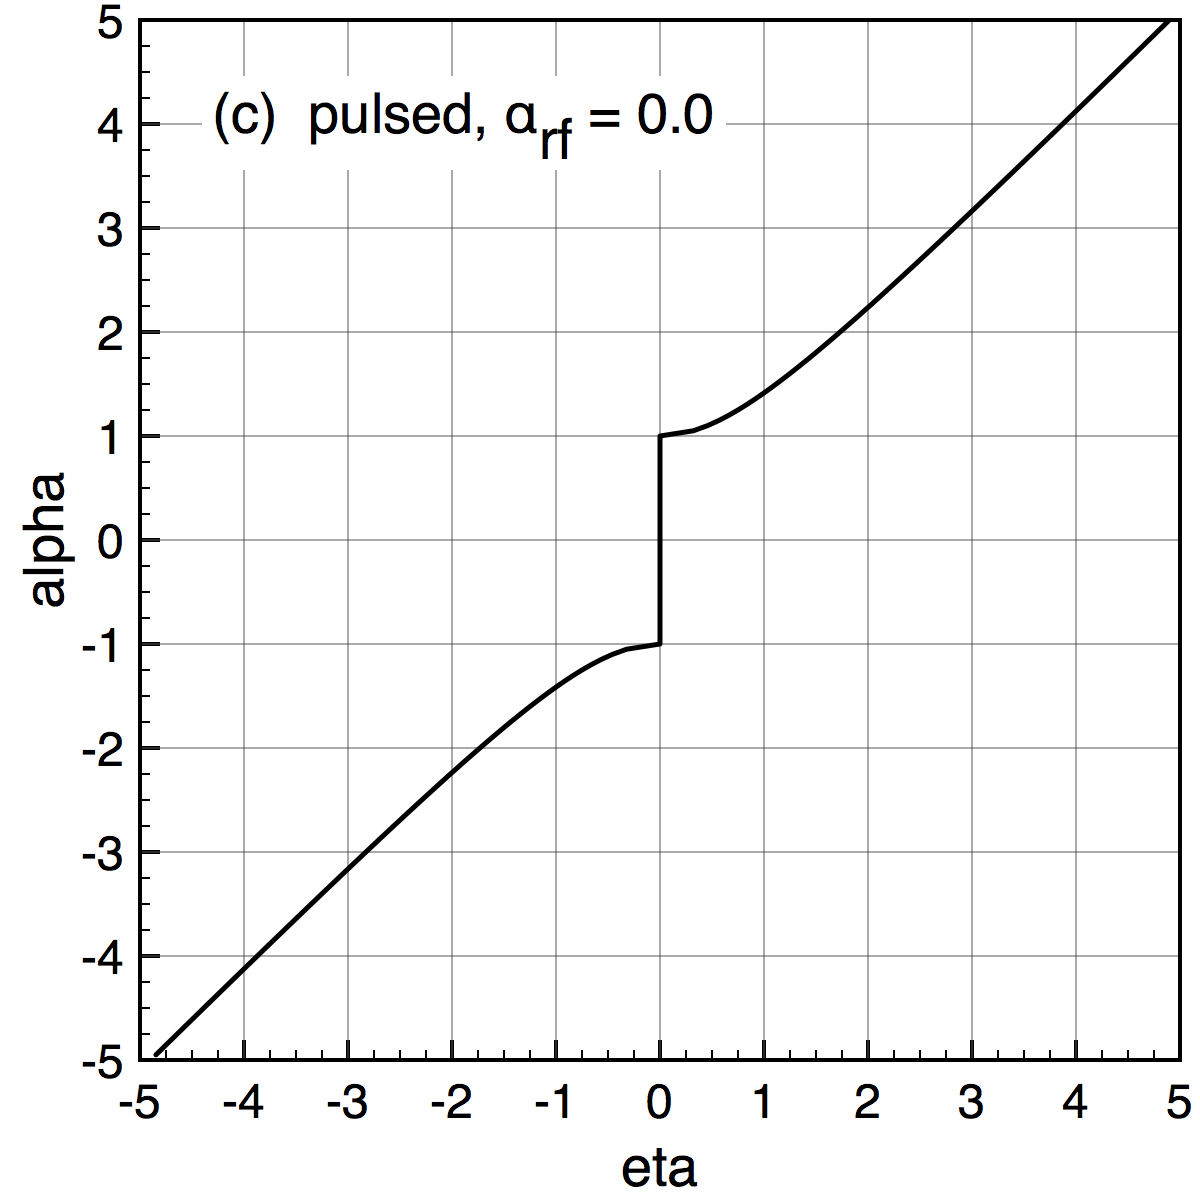
\includegraphics[width=0.325\textwidth]{iv-pulsed-alpharf0.png}}
%	\hfill
%	\mbox{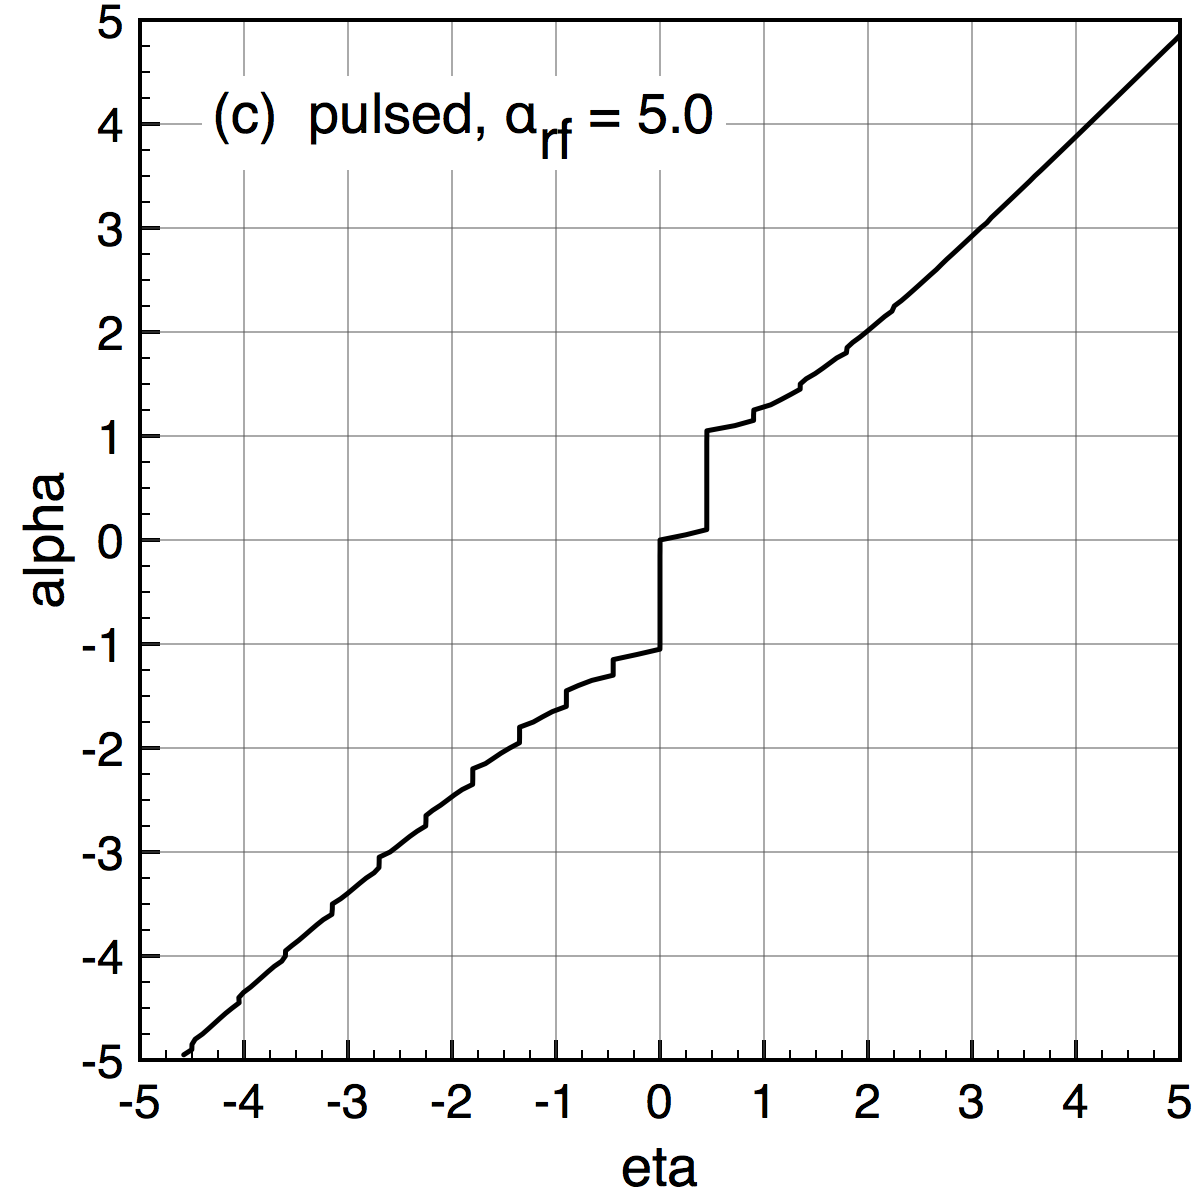
\includegraphics[width=0.325\textwidth]{iv-pulsed-alpharf5.png}}
%	\hfill
%	\mbox{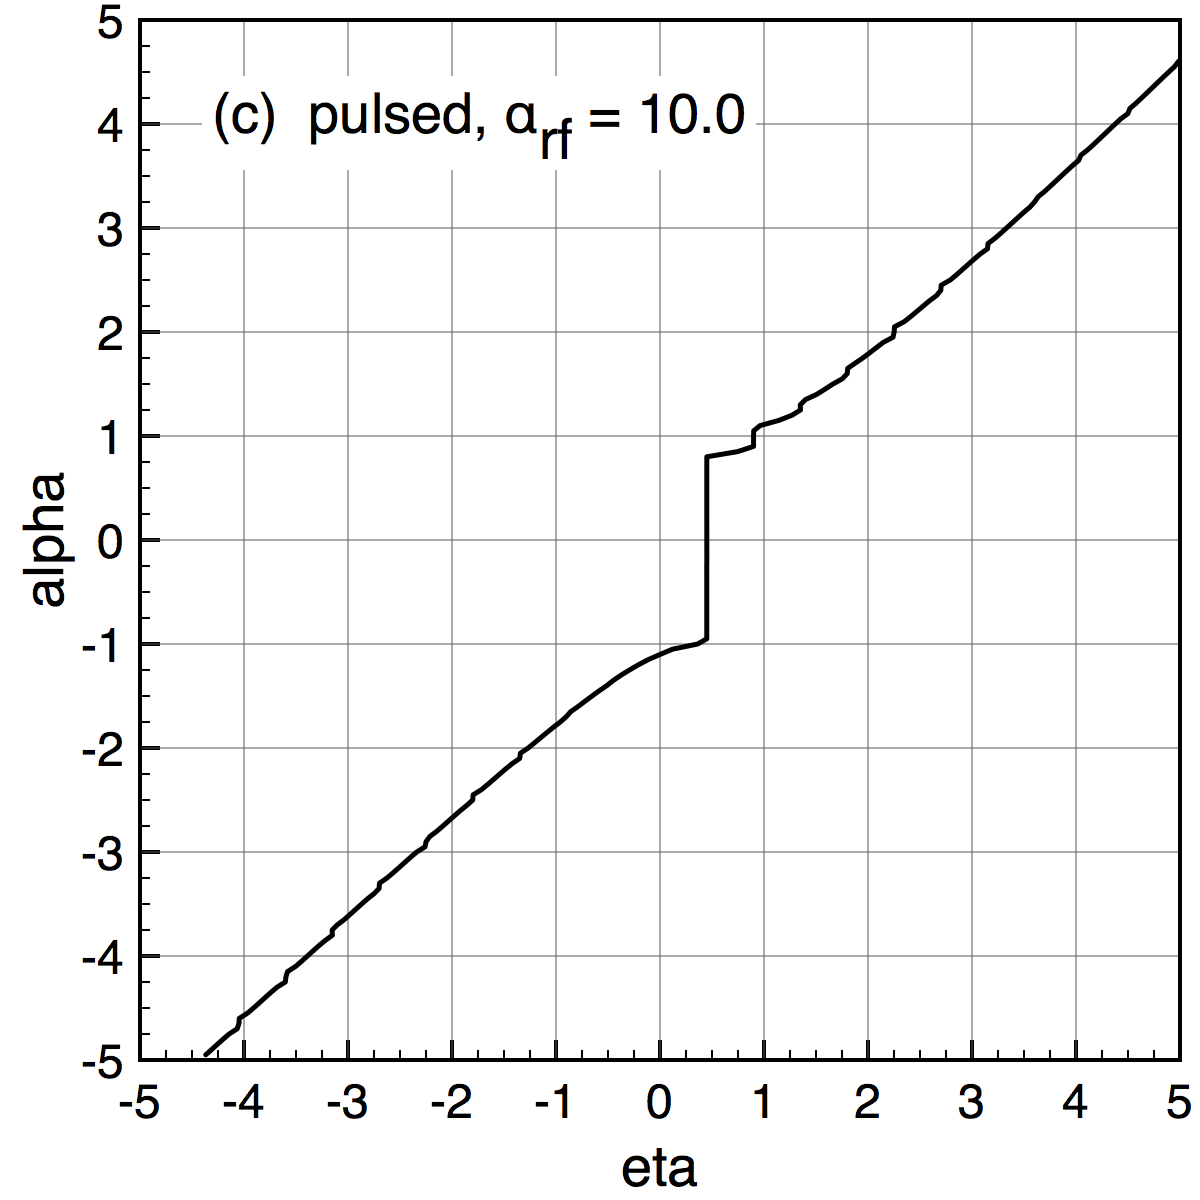
\includegraphics[width=0.325\textwidth]{iv-pulsed-alpharf10.png}}
%}
%	\caption{$I - V$ characteristics of a junction with $\beta_c = 0.01$, driven by a pulsed rf bias of frequency $\Omega = 0.45$ for: (a) $\alpha_\mathrm{rf} = 0.0$, (b) $\alpha_\mathrm{rf} = 5.0$ and (c) $\alpha_\mathrm{rf} = 10.0$. For $\alpha_\mathrm{rf} > 0$ the rf-induced steps are much larger than with the standard sinusoidal rf-drive. Here $\eta$ and $\alpha$ are the junction normalized voltage and current, respectively.}
%	\label{fig:iv-pulsed}
%\end{figure}
%%===============================================================================


%The second Fortran program, \texttt{mcp-work.for}, is much more interesting. While \texttt{mcphase.for} can calculate the $I - V$ characteristic of the junction only for a single value of $\alpha_\mathrm{rf}$ and for increasing or decreasing values of the normalized current $\alpha_\mathrm{dc}$, 
As already noted, \texttt{mcp-work.for} sweeps the normalized current $\alpha_\mathrm{dc}$ in both directions to help visualize the possible hysteresis of the junction and calculates the $I - V$ characteristics for a range of values of $\alpha_\mathrm{rf}$, saving each curve in a separate output file. 
The lower and upper limits and the step size of $\alpha_\mathrm{rf}$ are hardcoded in the Fortran source code ad every change requires a recompilation of \texttt{mcp-work.for} (a minor hassle, as the compilation takes just a couple of seconds on a modern machine).

Also the names of the output data files are hard-coded in the \texttt{mcp-work.for} in the \texttt{filewrite} variable and are conventionally composed by a two-letter prefix ("SI" for the single drive, "BI" for the biharmonic driva and "PU" for the pulsed drive) followed by a three-digit integer that represents the cycle number (Section~\ref{compilation-with-gfortran}).

To avoid cluttering the \texttt{mccumber/} directory containing the Fortran source files (Section~\ref{sec:digging-into-code}) with the output data files produced by the simulations, I created  a new directory, \texttt{2020runs/}, in the main project folder, where I copied the \texttt{mc-iv.dat} configuration file needed to start the simulation (Fig.~\ref{fig:source-header}).

Running \texttt{mcp-work.for} requires only three steps: compile \texttt{mcp-work.for} with the proper directives, switch to the \texttt{2020runs/} directory and run the \texttt{mcp-work} executable from there. The whole process is summarized below for the sinusoidal drive,

%===============================================================================
\lstset{
    language = bash,
    basicstyle = \small\bfseries\ttfamily,
    tabsize = 4,
    frame = none,
    framesep = 2em,
    framexleftmargin = 1em,
    backgroundcolor = \color{ultralightgray},
    keywordstyle = \color{darkred}\bfseries,
    alsoletter=-,
    morekeywords = {gfortran},
    deletekeywords = {for}
}
%===============================================================================
\begin{lstlisting}
$ gfortran -cpp -Dtextout -Dsingle -o mcp-work mcp-work.for
$ cd ../2020runs/
$ ../mccumber/mcp-work
\end{lstlisting}
%===============================================================================


The only modification needed to perform calculations using the pulsed drive is to change the \texttt{-Dsingle} directive to \texttt{-Dpulsed},

%===============================================================================
\begin{lstlisting}
$ gfortran -cpp -Dtextout -Dpulsed -o mcp-work mcp-work.for
$ cd ../2020runs/
$ ../mccumber/mcp-work
\end{lstlisting}
%===============================================================================


On a modern (but not state-of-the art) machine the whole simulation with $100 \alpha_\mathrm{rf}$ steps takes around $5 - 8$ minutes for the single drive and $7 -11$ minutes for the pulsed drive, and most of the time is spent printing on the terminal the calculated $I - V$ characteristics for each value of $\alpha_\mathrm{rf}$. Such feedback was useful at the time of the original calculation, as every new calculated point of the $I - V$ characteristics appeared on the screen after several tens of seconds, now the results scroll on the screen at a speed that makes them almost illegible.
However, to keep as faithful as possible to the original project, I decided to continue to print the data points on the computer screen.

I also briefly tried to compile the original Fortran code with the Microsoft Fortran 5.1 installed in the emulator. Compilation was fine but the resulting DOS program was extremely slow, taking about $55$ seconds for each $\alpha_\mathrm{rf}$ cycle and about $90$ minutes in total for the sinusoidal drive, more than a tenfold increase with respect to the native macOS version compiled with gfortran.
Even considering the overhead of the emulator, the difference is too large not to be attributed to the low quality of the binary code generated by the Microsoft Fortran 5.1 compiler.

The $I - V$ characteristics calculated with the sinusoidal drive are shown in Fig.~\ref{fig:iv-single} for different values of $\alpha_\mathrm{rf}$.
Without microwave radiation ($\alpha_\mathrm{rf} = 0$), the simulation produces well-known non-hysteretic $I - V$ characteristic of the RSJ model (Fig.~\ref{fig:iv-single}a), while for non-zero values of $\alpha_\mathrm{rf}$ the staircase-like structure of the rf-induced current steps appear on the $I - V$ curves (Fig.~\ref{fig:iv-single}b and Fig.~\ref{fig:iv-single}c).

%===============================================================================
\begin{figure}[tb]
{
	\fboxsep=0pt
	\mbox{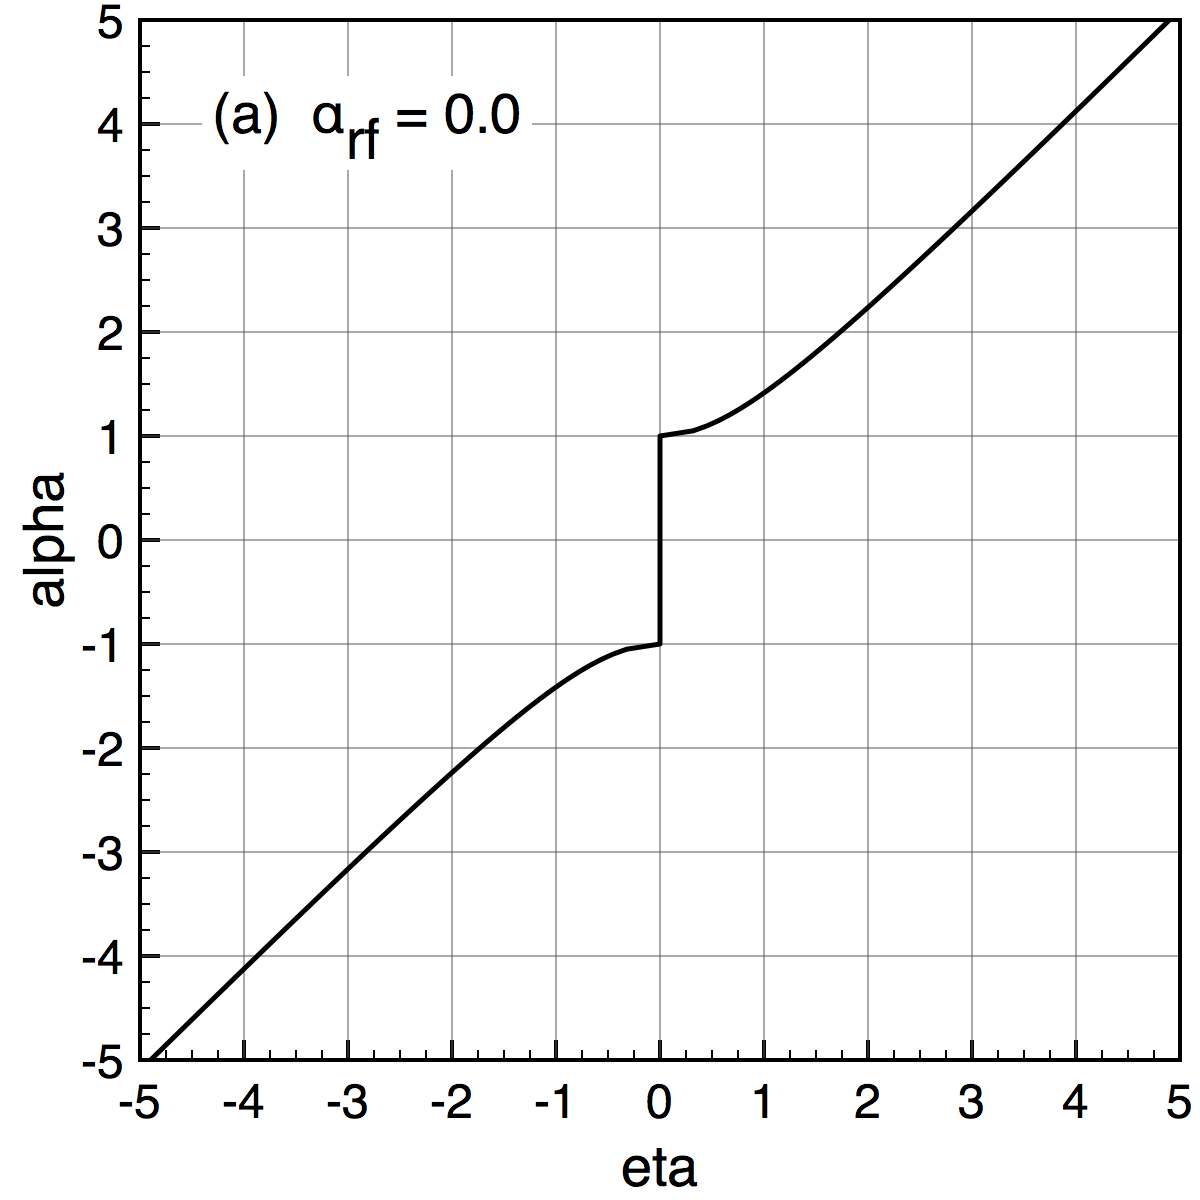
\includegraphics[width=0.325\textwidth]{iv-single-alpharf0.png}}
	\hfill
	\mbox{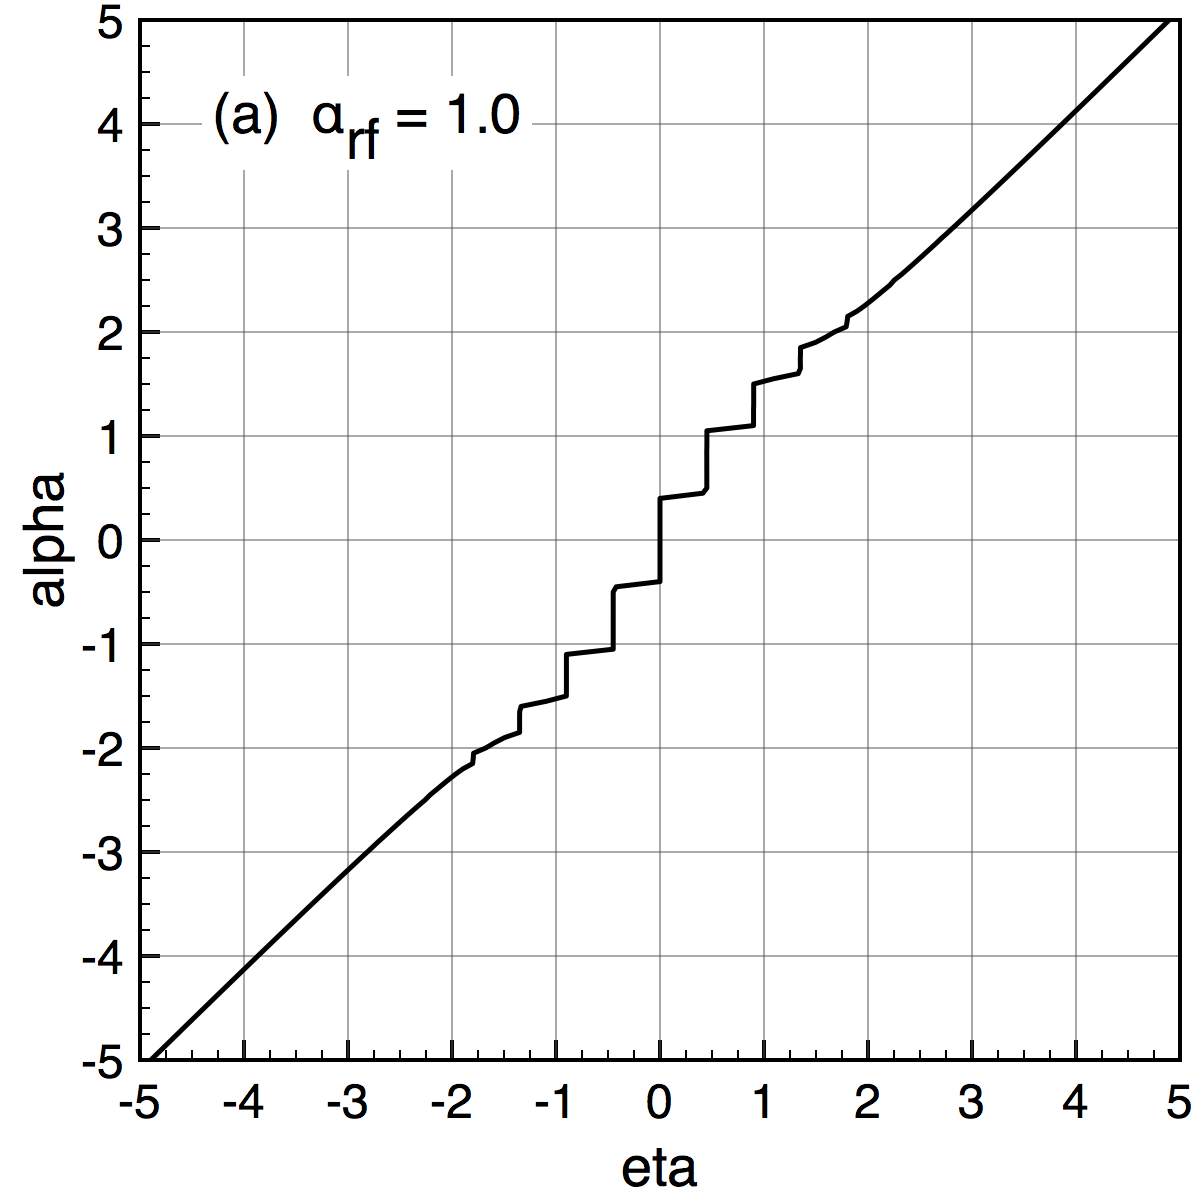
\includegraphics[width=0.325\textwidth]{iv-single-alpharf1.png}}
	\hfill
	\mbox{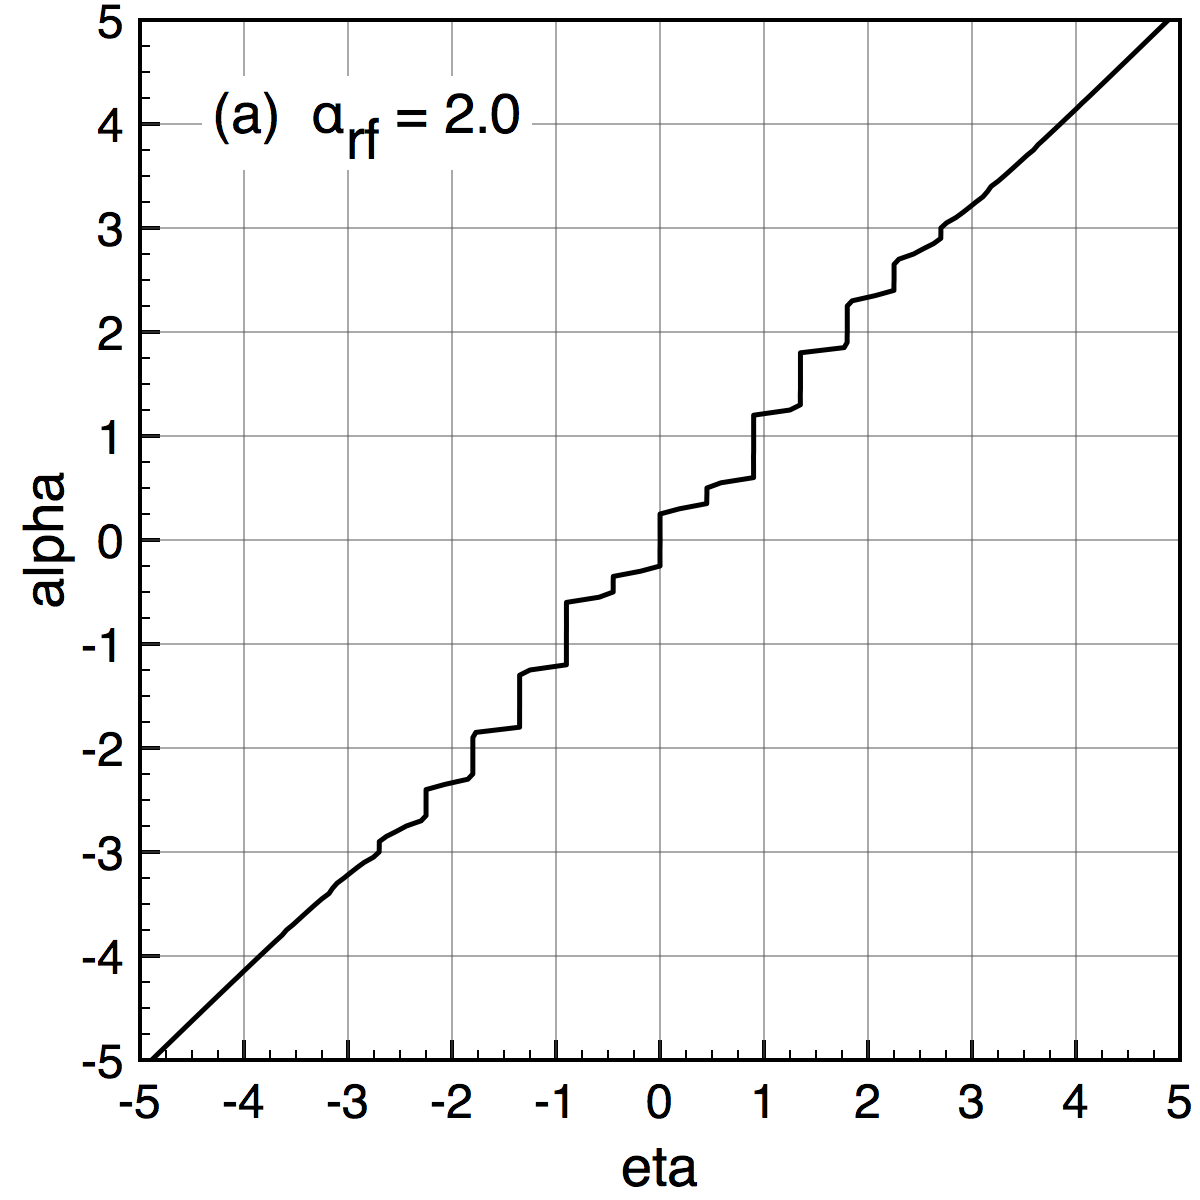
\includegraphics[width=0.325\textwidth]{iv-single-alpharf2.png}}
}
	\caption{$I - V$ characteristics of a junction with $\beta_c = 0.01$, driven by a sinusoidal rf bias of frequency $\Omega = 0.45$ and (a) $\alpha_\mathrm{rf} = 0.0$, (b) $\alpha_\mathrm{rf} = 1.0$ and (c) $\alpha_\mathrm{rf} = 2.0$. The rf-induced current steps are clearly visible when $\alpha_\mathrm{rf} > 0$. Here $\eta$ and $\alpha$ are the junction normalized voltage and current, respectively.}
	\label{fig:iv-single}
\end{figure}
%===============================================================================


For a pulsed drive, the $I - V$ characteristic without microwave radiation is identical to that calculated with the sinusoidal signal (Fig.~\ref{fig:iv-pulsed}a), while the current steps induced by the pulsed drive are fewer and nearly as wide as the critical current for $\alpha_\mathrm{rf} = 0.0$ (compare Figs.~\ref{fig:iv-pulsed}a and \ref{fig:iv-pulsed}c).

%===============================================================================
\begin{figure}[tb]
{
	\fboxsep=0pt
	\mbox{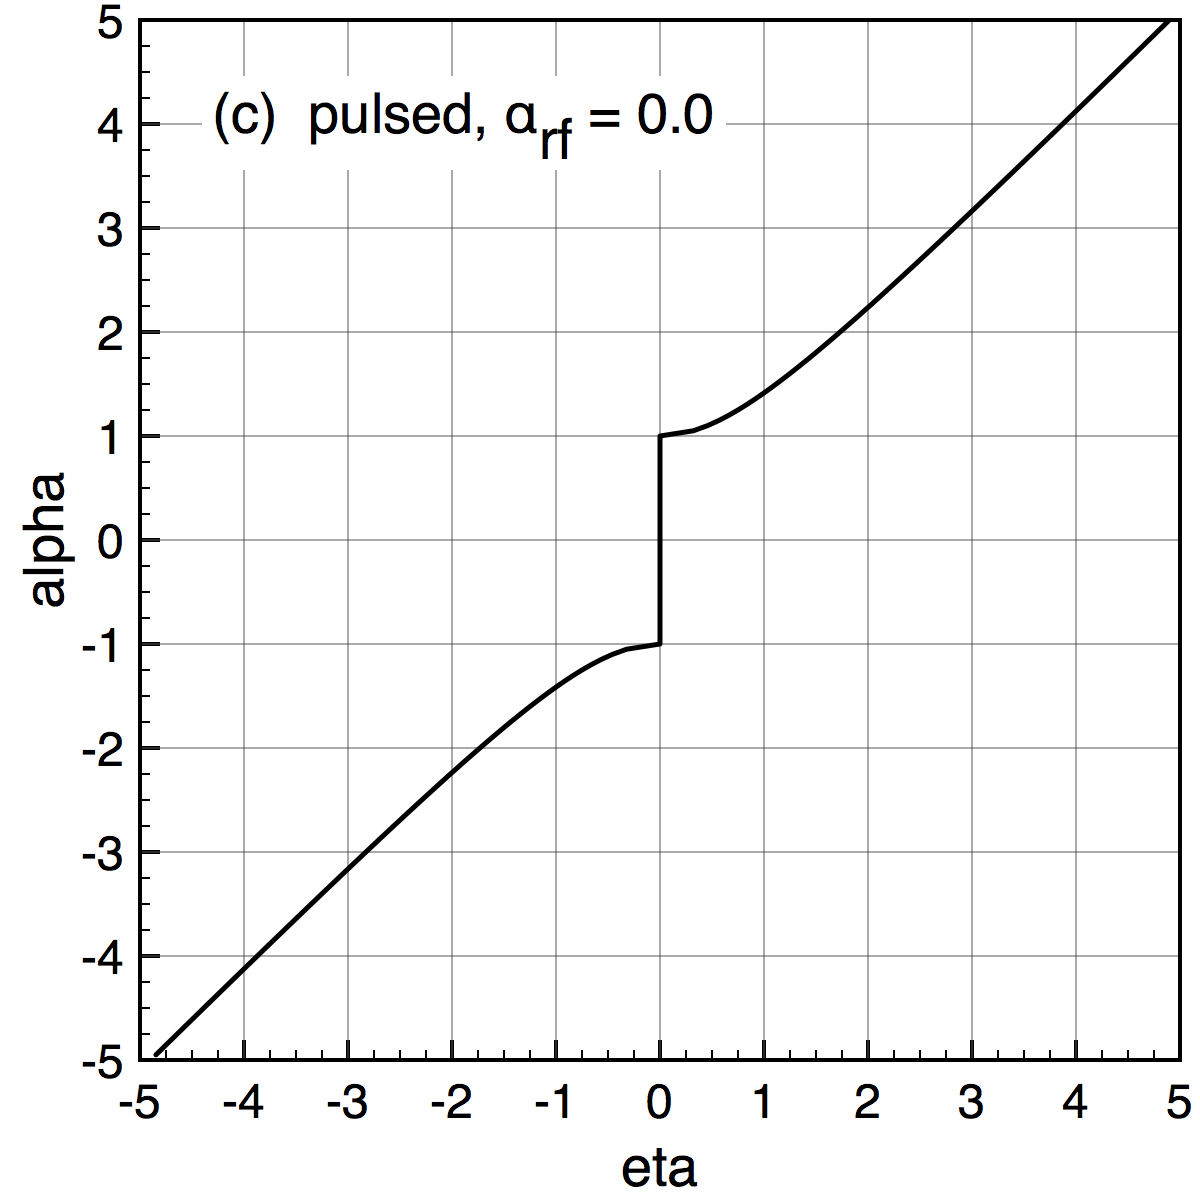
\includegraphics[width=0.325\textwidth]{iv-pulsed-alpharf0.png}}
	\hfill
	\mbox{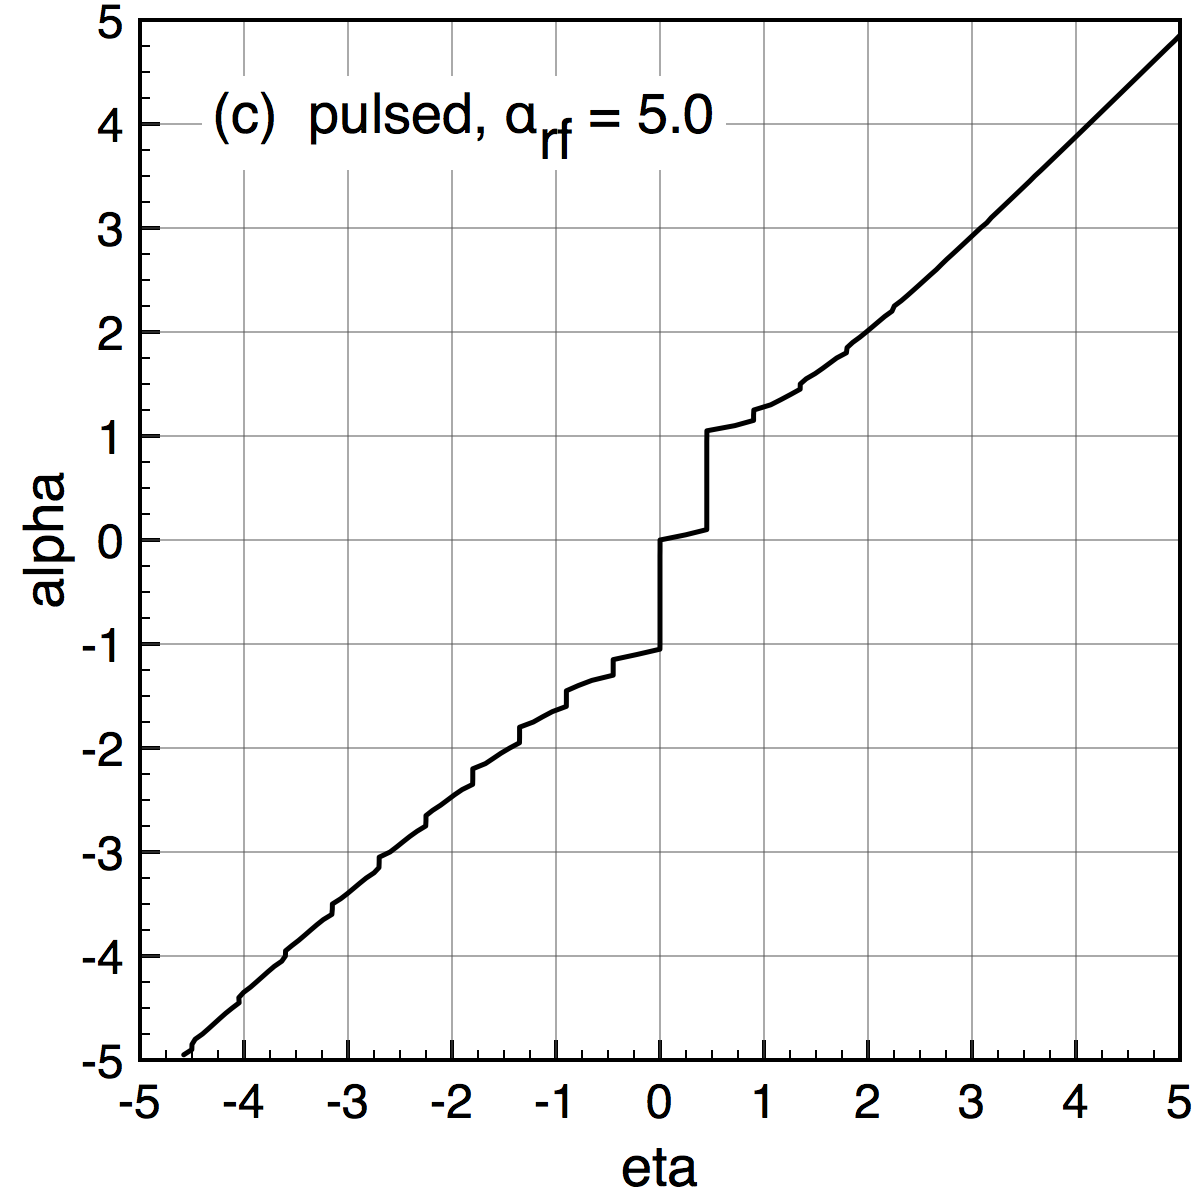
\includegraphics[width=0.325\textwidth]{iv-pulsed-alpharf5.png}}
	\hfill
	\mbox{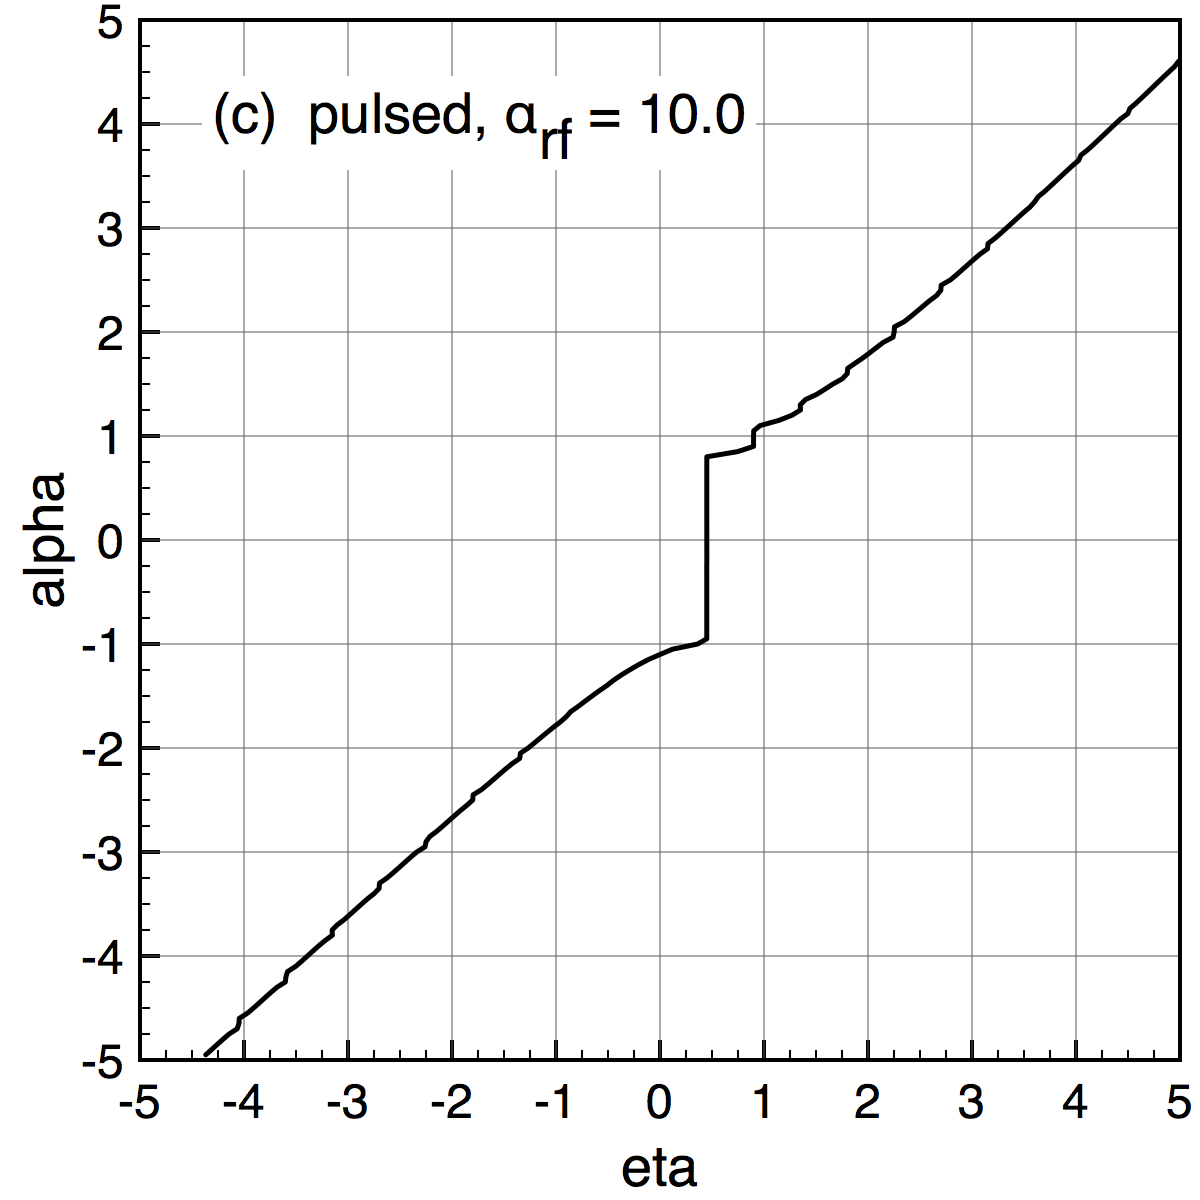
\includegraphics[width=0.325\textwidth]{iv-pulsed-alpharf10.png}}
}
	\caption{$I - V$ characteristics of a junction with $\beta_c = 0.01$, driven by a pulsed rf bias of frequency $\Omega = 0.45$ for: (a) $\alpha_\mathrm{rf} = 0.0$, (b) $\alpha_\mathrm{rf} = 5.0$ and (c) $\alpha_\mathrm{rf} = 10.0$. For $\alpha_\mathrm{rf} > 0$ the rf-induced steps are much larger than with the standard sinusoidal rf-drive. Here $\eta$ and $\alpha$ are the junction normalized voltage and current, respectively.}
	\label{fig:iv-pulsed}
\end{figure}
%===============================================================================


At the end of each run, the output files must be transferred to the Windows 3.11 virtual machine to be processed by \texttt{stepampl}, the Visual Basic application described in Section~\ref{visual-basic-code}. However Windows 3.11 does not \emph{understand} Unix line terminators and cannot read the output files without a preliminary conversion. 
This conversion can be easily done in the macOS Terminal with the following command

%===============================================================================
\lstset{
    language = bash,
    basicstyle = \small\bfseries\ttfamily,
    tabsize = 4,
    frame = none,
    framesep = 2em,
    framexleftmargin = 1em,
    backgroundcolor = \color{ultralightgray},
    keywordstyle = \color{darkred}\bfseries,
    alsoletter=;,
    morekeywords = {;},
}
%===============================================================================
\begin{lstlisting}
$ for f in $(ls *.out); do sed -i .bak s/$/$'\r'/ $f ; done
\end{lstlisting}
%===============================================================================

that changes the line terminators of the \texttt{.out} output files from the Unix format containing only a line-feed (LF) to the carriage return followed by a line-feed (CR-LF) format used by all versions of Microsoft Windows. 
\footnote{Slightly different versions of the command can be found on the internet; the format used above is POSIX-compliant and should run on any Unix flavour}.
The \texttt{-i} switch allows in-place conversion of each file, the original files are kept with a \texttt{.bak} extension.

After conversion the output files in the proper Windows compatible format can be transferred onto the virtual floppy disk image. %virtual floppy disk image can be mounted on the Desktop of the host operating system by double-clicking on its icon and the output files in the proper Windows format can be transferred onto the virtual floppy disk. 
When the transfer is done, the floppy disk image is unmounted from the host operating system and mounted  in the virtual machine, making it visible to Windows 3.11. 
The output files are copied to an empty directory of Windows 3.11 and the Visual Basic application is started, either by running the precompiled \texttt{stepampl.exe} application or by opening the Visual Basic project and running the program from there (Fig.~\ref{fig:stepampl}), that calculates the size of the quantized current steps for each value of $\alpha_\mathrm{rf}$ and saves the results in another text file with extension \texttt{.STP} (for steps) that could be transferred back to the host operating system via the virtual floppy disk image.

[++ TOGLIERE? The original Visual Basic code had a hard coded limit set to a maximum number of $100$ processed files. This limit was probably related to memory problems or simply to the fact that it was impossible to run an overnight simulation with more than $100$ different $\alpha_\mathrm{rf}$ values. ++]

%%===============================================================================
%\begin{figure}[tbh]
%	\centering
%	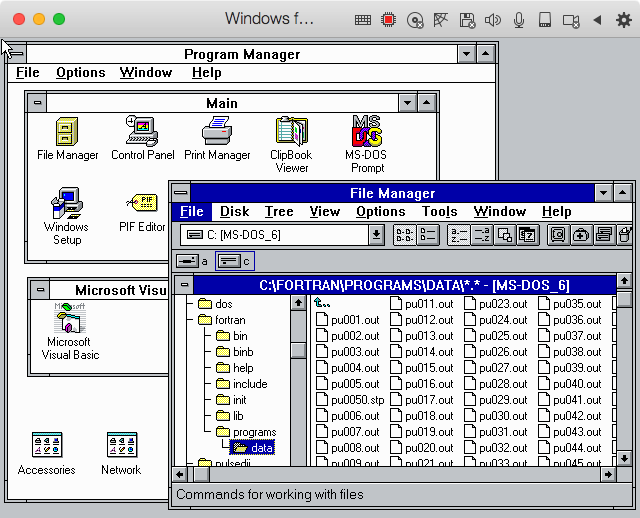
\includegraphics[width=0.75\textwidth]{windows-311.png}
%	\caption{Windows 3.11 desktop showing the program \texttt{stepampl} that has just finished to process the data files.}
%	\label{fig:stepampl}
%\end{figure}
%%===============================================================================


At the time of writing the original paper \cite{Maggi:1996}, the whole process had to be repeated each night for a different set of input parameters  and for a different kind of microwave signal (single, biharmonic or pulsed).

Each night I used three of the available DEC workstations to simulate in parallel the junction behavior with the pulsed drive, with three different values of the (normalized) width of the pulse signal, $\rho$, while keeping constant all the other parameters, such $\beta$ and $\Omega$.
The only other difference in these simulation was the range of variation of $\alpha_\mathrm{rf}$, which depended on the value of $\rho$ (shorter pulses require a much larger intensity of the rf-signal to have the same effect on the junction).
The fourth machine simulated the junction behavior with the standard sinusoidal drive, using exactly the same set of junction parameters.
%Each night a different set of junction parameters was used.

The original paper  contained all the information needed to reproduce the results shown in the figures, without having to repeat the whole analysis from scratch. 
The parameters used in all runs were: hysteresis parameter $\beta = 0.01$, frequency of the sinusoidal or pulsed  rf signal $\Omega = 0.45$, normalized current bias between $\alpha_\mathrm{dc} = -5.0$ and $\alpha_\mathrm{dc} = 5.0$, normalized integration time $\tau = 500$ with step $\Delta \tau = 0.01$. 

The simulation with the sinusoidal drive was performed by varying the amplitude of the rf signal $\alpha_\mathrm{rf}$ between $0.0$ and $5.0$, with a step $\Delta \alpha_\mathrm{rf} = 0.05$.
The three simulations with the pulsed drive were done using: 
(1) pulse width $\rho = 0.250$, $\alpha_\mathrm{rf} = 0.0 - 10.0$, $\Delta \alpha_\mathrm{rf} = 0.1$;
(2) pulse width $\rho = 0.125$, $\alpha_\mathrm{rf} = 0.0 - 20.0$, $\Delta \alpha_\mathrm{rf} = 0.2$;
(3) pulse width $\rho = 0.050$, $\alpha_\mathrm{rf} = 0.0 - 50.0$, $\Delta \alpha_\mathrm{rf} = 0.5$.

The resulting output and summary files were saved in separate folders in the \texttt{2020runs/} directory, named \texttt{SINGLE/}, \texttt{PULS0250}, \texttt{PULS125}, \texttt{PULS0050} after their DOS counterparts.

To reproduce the first and second figure of \cite{Maggi:1996} I made the only concession to modernity. instead of trying to recreate them with the plotting program used originally, probably \href{https://www.originlab.com}{Origin 2.0}, I decided to write a couple of small R scripts that could automate the task.
The results are shown in Fig.~\ref{fig:pulsed-ivs} and Fig.~\ref{fig:step-width} and, as expected, are identical to those reported in the first two figures of \cite{Maggi:1996}. 
Figure 3 of the original paper could be easily reproduced by plotting the maxima of the curves of Fig.~\ref{fig:step-width}, i.e., $\Delta i_n$ vs. $\alpha_\mathrm{rf}$, for the four different cases considered here.
Note that the large vertical steps on the rightmost curves of Fig.~\ref{fig:pulsed-ivs} era the first rf-induced steps, that can be nearly as large as the critical current $I_C$ without rf bias visible in the first plot on the left.

%===============================================================================
\begin{figure}[t]
	\centering
	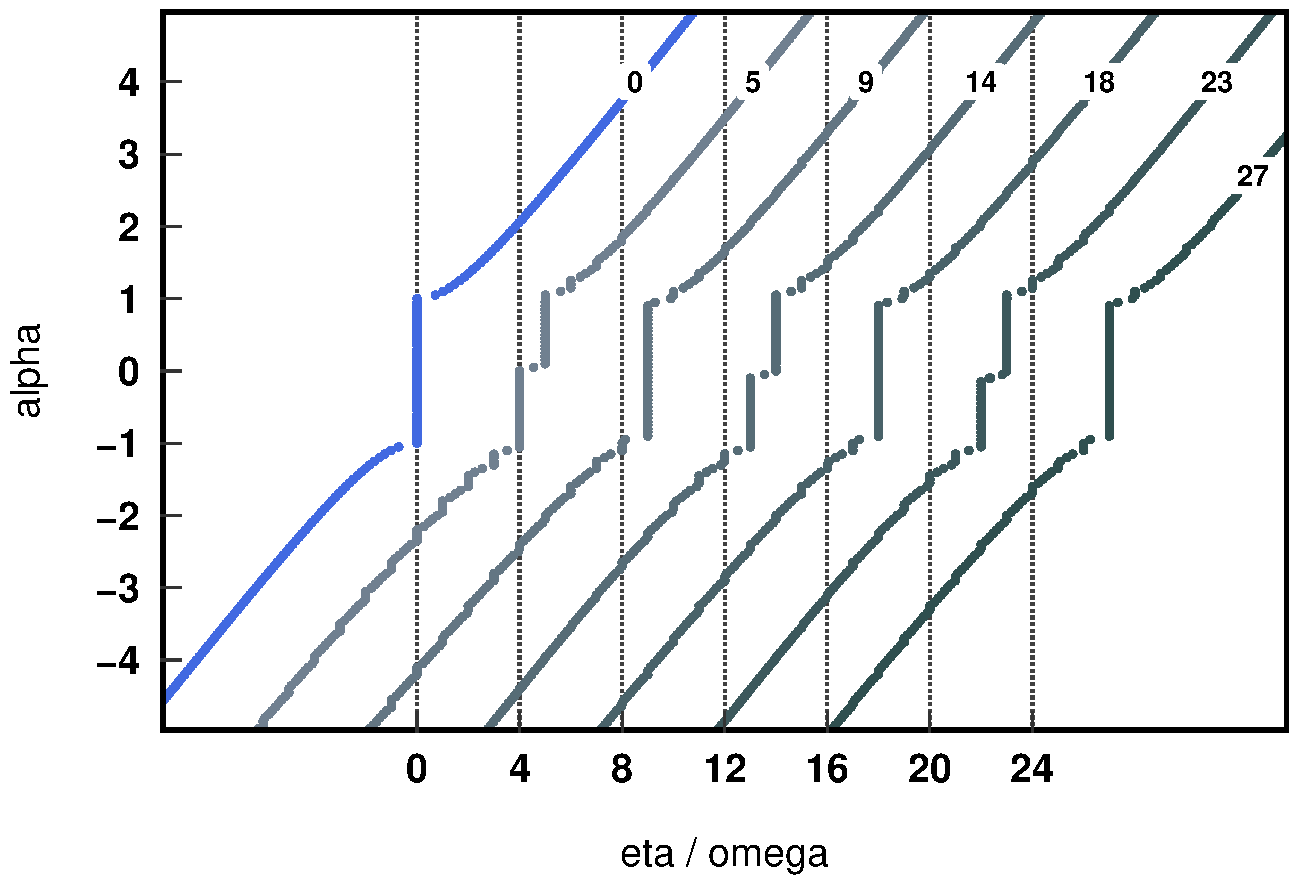
\includegraphics[width = 0.75 \textwidth]{PULS0050-IV.pdf}
	\caption{$I - V$ curves of a junction with $\beta = 0.01$ for several values of the rf bias. The junction is  irradiated by a train of rf pulses of repetition frequency $\Omega = 0.45$ and pulse duration $\rho = 0.05$. Each curve has been offset horizontally by $4 \Omega$. The vertical dotted lines mark the position of the zero-voltage axis for the $I - V$ curve located immediately to the right.}
	\label{fig:pulsed-ivs}
\end{figure}
%===============================================================================


%%===============================================================================
%\begin{figure}[h]
%{
%	\fboxsep=0pt
%	\mbox{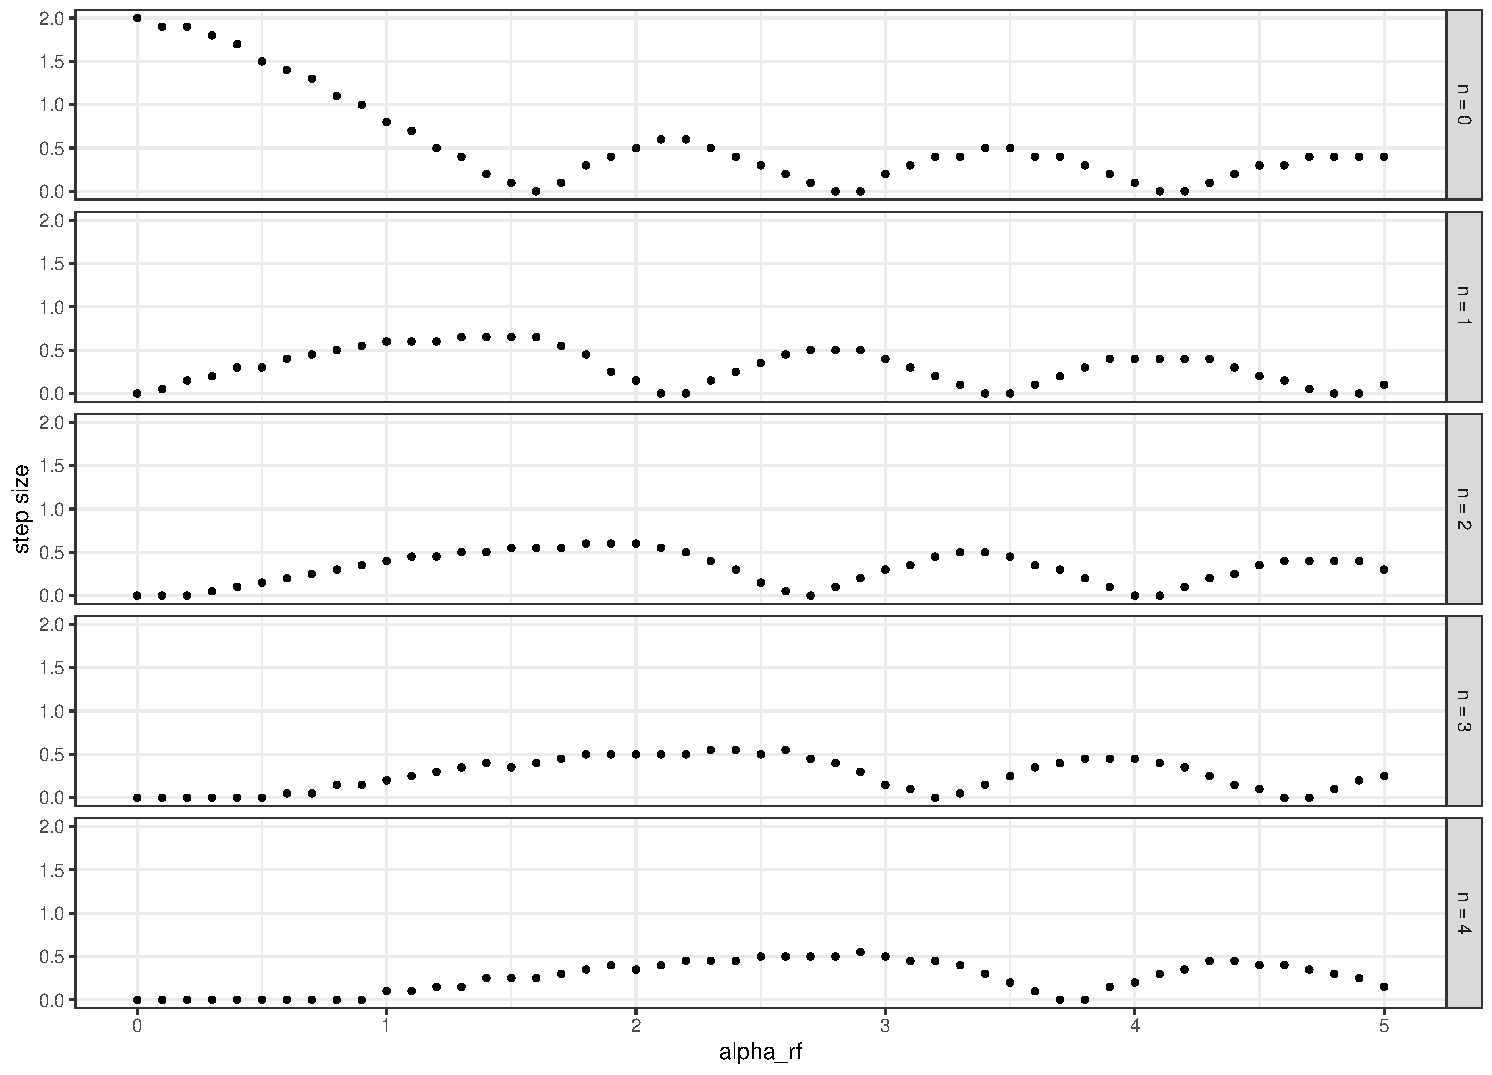
\includegraphics[width=0.45\textwidth]{SINGLE.pdf}}
%	\hfill
%	\mbox{\includegraphics[width=0.45\textwidth]PULS0250.pdf}}
%}
%%{
%%	\fboxsep=0pt
%%	\mbox{\includegraphics[width=0.45\textwidth]PULS0250.pdf}}
%%	\hfill
%%	\mbox{\includegraphics[width=0.45\textwidth]PULS0050.pdf}}
%%}
%	\caption{.}
%	\label{fig:step-width}
%\end{figure}
%%===============================================================================
%===============================================================================
\begin{figure}[!p]
	\centering
	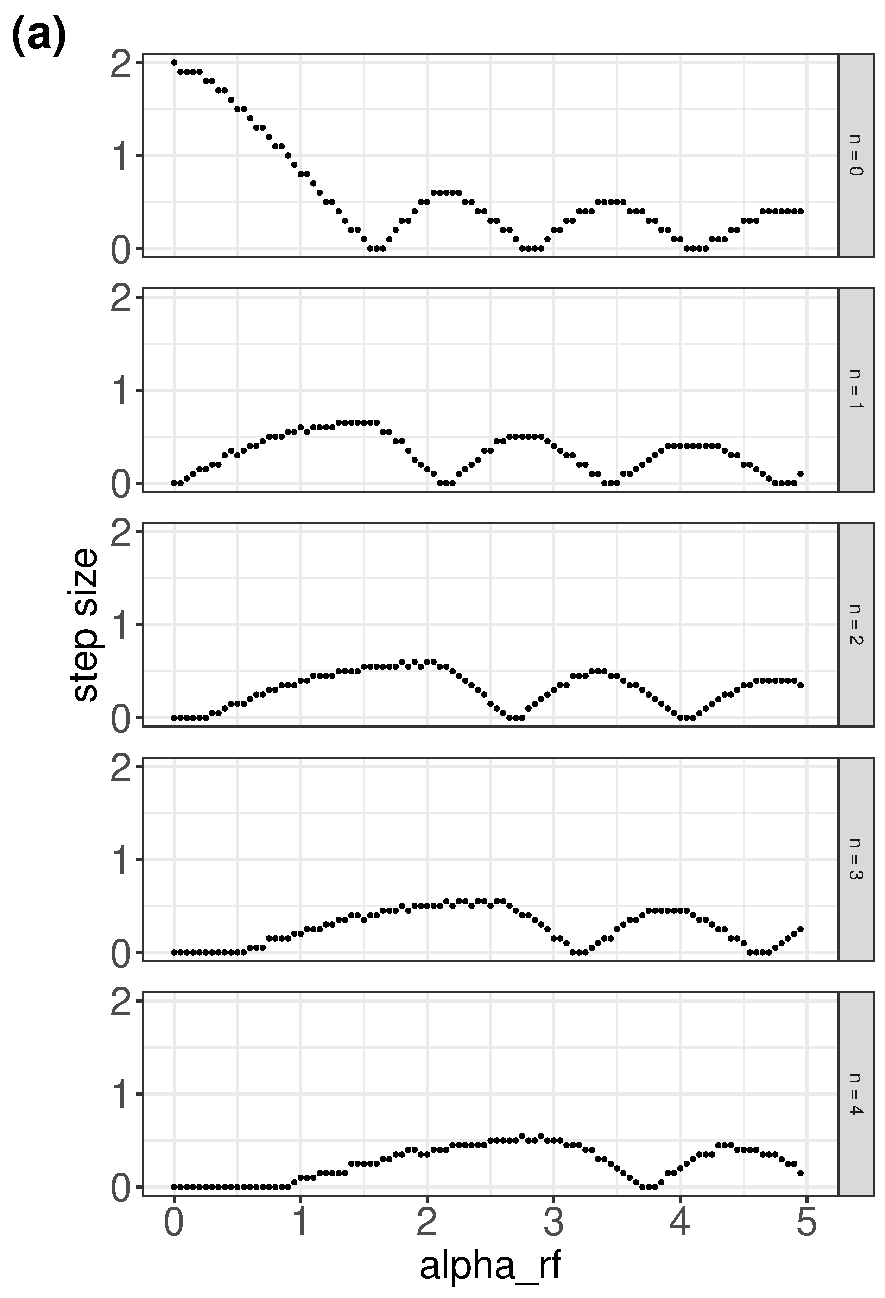
\includegraphics[width=0.45\textwidth]{SINGLE2.pdf}
	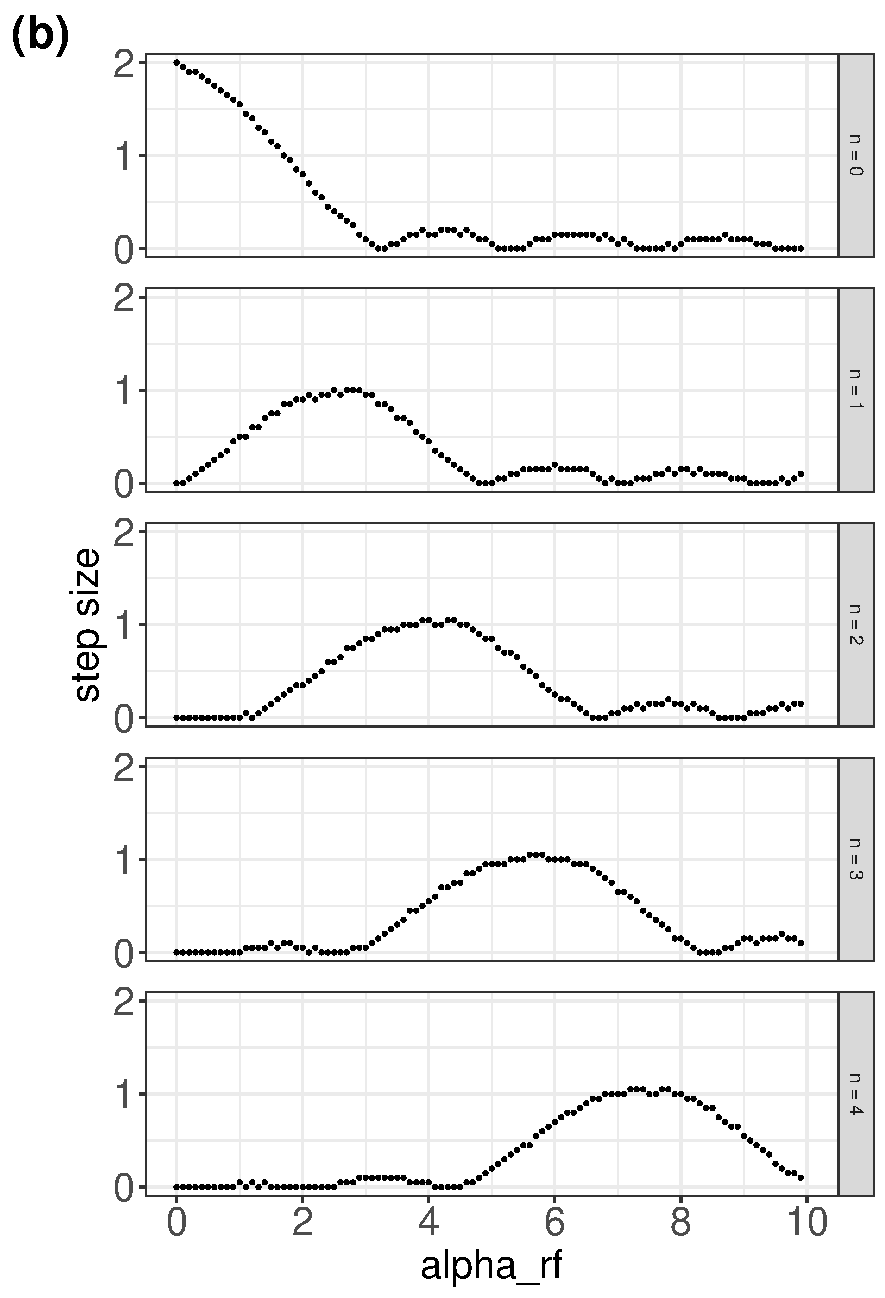
\includegraphics[width=0.45\textwidth]{PULS0250.pdf}
	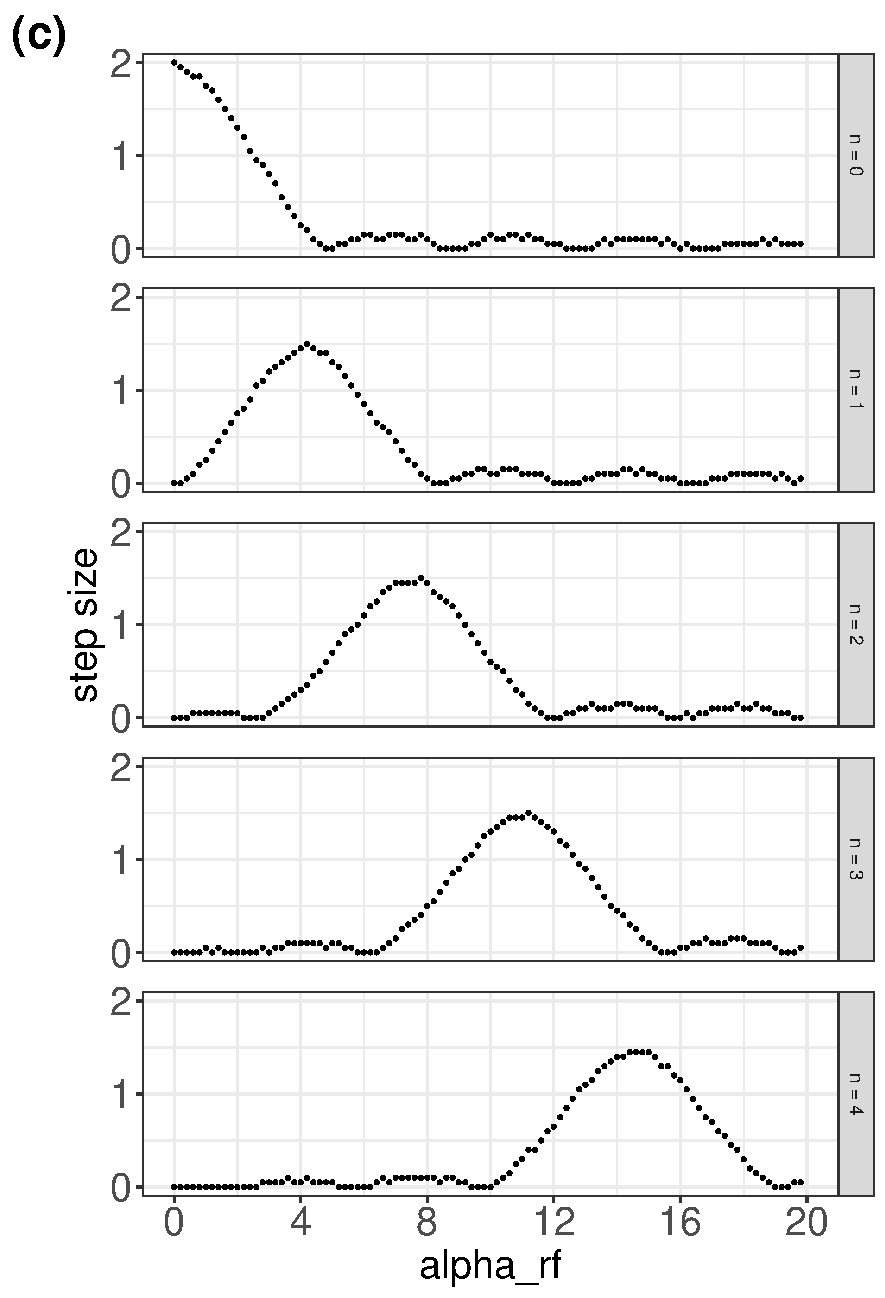
\includegraphics[width=0.45\textwidth]{PULS0125.pdf}
	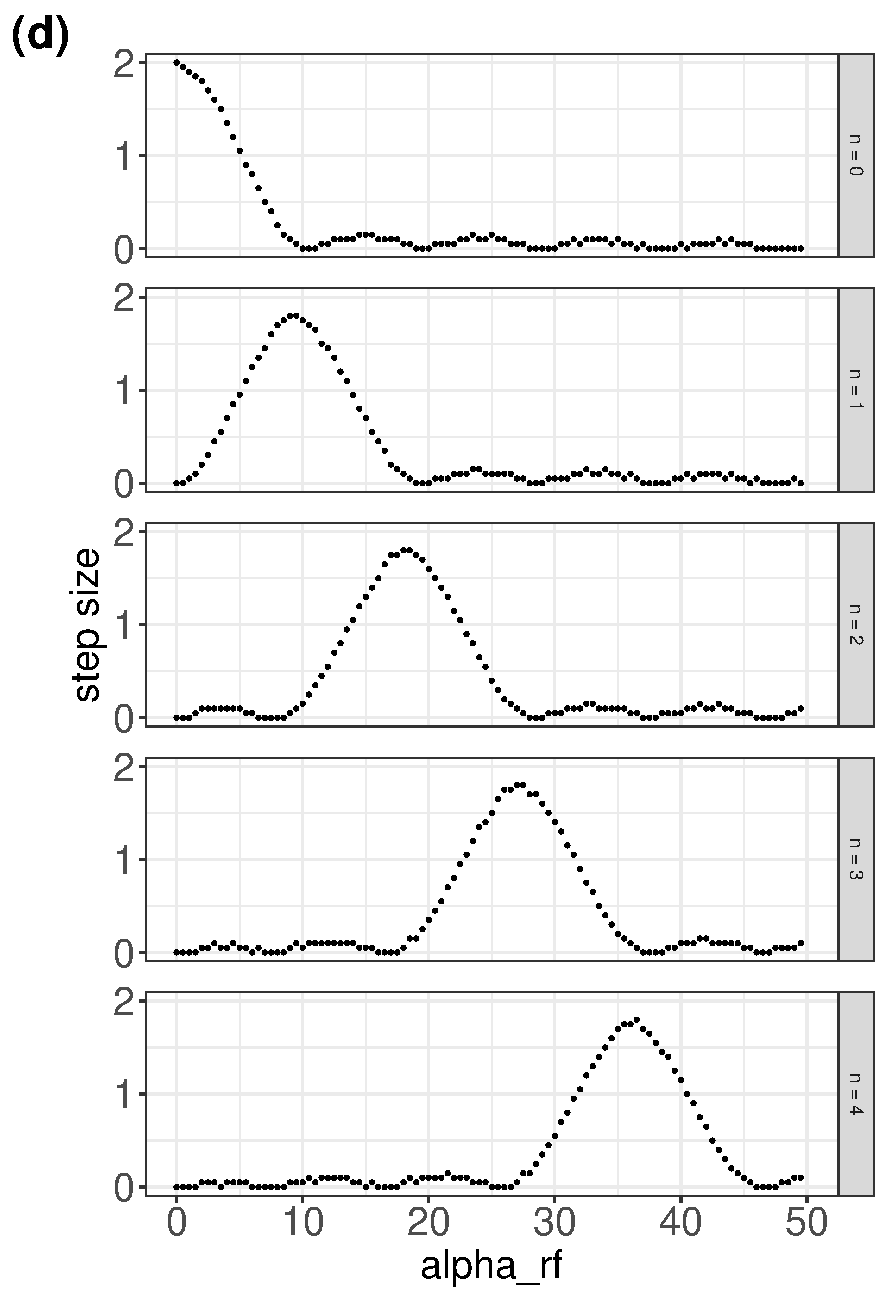
\includegraphics[width=0.45\textwidth]{PULS0050.pdf}
	\caption{Dependence of the step size $\Delta i_n$ on the amplitude of  $\alpha_\mathrm{rf}$, for $n = 0. . . 4$. The $n = 0$ step is the normalized total critical current $\Delta i_0$ of the junction. The junction parameters are $\beta = 0. 01$ and $\Omega = 0. 45$; (a) sinusoidal drive, (b) pulsed drive with $\rho = 0. 250$, (c) pulsed drive with $\rho = 0. 125$, (d) pulsed drive with $\rho = 0. 050$.}
	\label{fig:step-width}
\end{figure}
%===============================================================================

%===============================================================================
\begin{figure}[t]
	\centering
	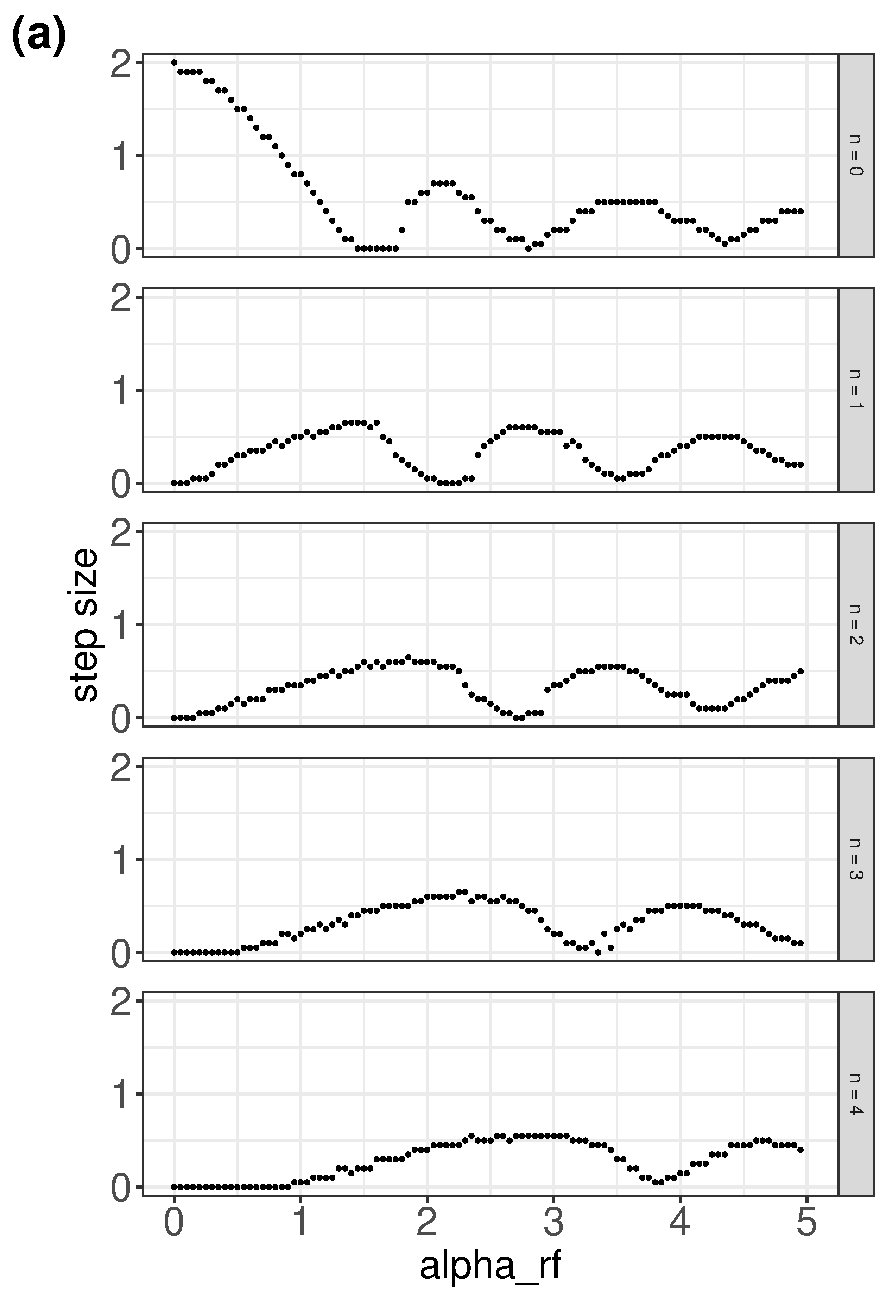
\includegraphics[width=0.45\textwidth]{SINGLE-BETA1.pdf}
	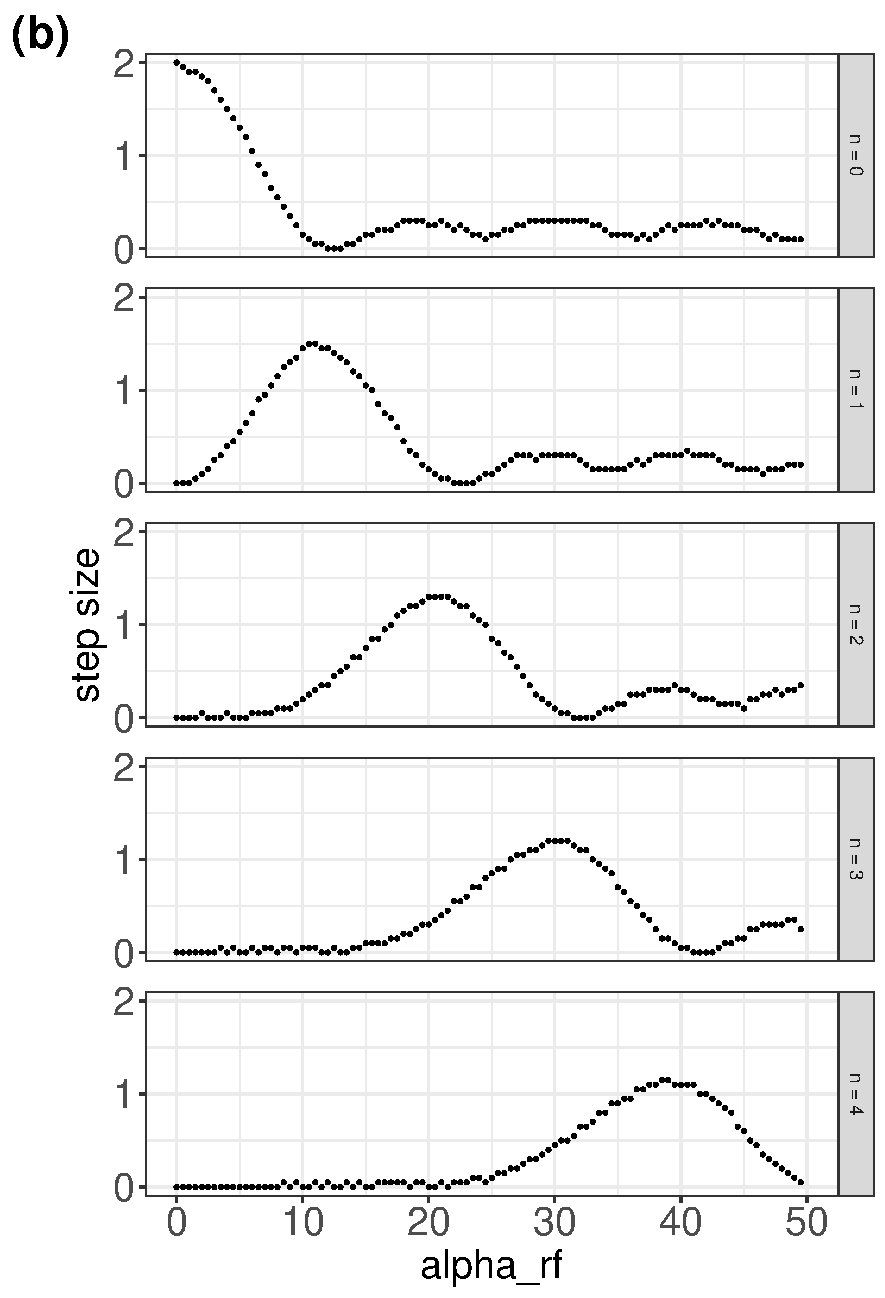
\includegraphics[width=0.45\textwidth]{PULS0050-BETA1.pdf}
	\caption{Dependence of the step size $\Delta i_n$ on the amplitude of  $\alpha_\mathrm{rf}$, for $n = 0. . . 4$. The $n = 0$ step is the normalized total critical current $\Delta i_0$ of the junction. The junction parameters are $\beta = 1.0$ and $\Omega = 0. 45$; (a) sinusoidal drive, (b) pulsed drive with $\rho = 0. 050$.}
	\label{fig:step-width-beta1}
\end{figure}
%===============================================================================

Similar considerations can be made for the reproduction of Figure 4 of the original paper, which considers a slightly hysteretic junction with $\beta = 1.0$. In the spirit of this challenge I have chosen to show instead [++ the $I - V$ curves of the simulated junction with $\beta = 1.0$ and ++] the related $\Delta i_n$ vs. $\alpha_\mathrm{rf}$ curves for the two most significant cases of rf bias, i.e., the sinusoidal drive and the pulsed drive with $\rho = 0.050$ (Fig.~\ref{fig:step-width-beta1}).



\section{Discussion}

The main problem with this reproduction work was the accidental loss of all my handwritten notes about the project, that compelled me to recover all information from the source and data files only. 
Keeping good and updated documentation about any research project is paramount, but equally important is to store all documentation in a safe location, where it can be easily retrieved.
Today most documents are in electronic form, making them even more prone to data loss whenever a disaster strikes.

Implementing a good and reliable backup strategy on different forms of storage media should be a mandatory requirement of any research project today, and this strategy should always combine local backups with backups on secondary storage locations physically well separated from the original data source. 

Starting the project today from scratch I would make very different choices about the programming languages to use for the simulation and data analysis steps.

Fortran, despite its venerable age, is still an excellent language for scientific programming, but today my language of choice for numerical computations is Python, because of its flexibility, ease of use, and  availability of excellent numerical libraries, such as NumPy and SciPy.

The main problems with Python are related to the tumultuous development of the language itself and of the thousands of available modules, which can cause incompatibilities even with code developed a few years ago. This problem can be, at least temporarily, be solved by using virtual environments, but a better standardized solution is strongly needed.
Another problem is related to its nature of interpreted language. However, the presence of well-documented Fortran and C bindings, can enhance performance of time-critical sections of code.

Today I would also avoid using a new language, as was Visual Basic 1.0 at the time (or as is Apple's Swift today) for a scientific project. 
It is true that in 1993-94 it would have been very hard to foresee the rapid demise of Microsoft's Visual Basic, nevertheless using a programming language only when at least it main core is stable, runs on a wide array of operating systems and is accepted by a wide community of developers is surely a safer bet.
%Data analysis today is usually made with R or Python (or to a much lesser extent, Julia or Scala), both open source tools running on all major operation systems, that predictably will be still available in the next 10 or even 20 years.

Not every software project can afford to be as stable as \TeX, the scientific typesetting system invented by the prominent mathematician and computer scientist Donald E. Knuth, that has reached a state where ``it is unwise to make further \emph{improvements} to the system [..] which should give the same results 100 years from now that they produce today'' \cite{Knuth:1990}.
But on the other hand, a development environment that changes too much and too often or that is subjected to the whims of a single software company creates more problems than it solves. 



\section{Conclusions}

Going back to my old paper has been an exceptionally interesting and instructive experience and I thank the organizers of this challenge for the opportunity offered.

However this is not only a nostalgic attitude. The reproducibility crisis is a serious issue today \cite{Miyakawa:2020}, that undermines scientific credibility and impacts the public's trust in science, paving the way to all sorts of fake and unscientific beliefs.
Being able to go back and reproduce what has been done in the past could ease the retraction of published papers containing fabricated, falsified, or modified data or results and could contribute to an easier identification of future frauds.

This of course requires to share and make freely available the original data and the tools used to analyze them. A few years ago this requirement was impossible to fulfill in practice. The digital world in which we live makes it almost inevitable.



%===============================================================================
%Among the things that might be interesting is:
%
%How did you conserve the sources
%Did you take care of registering RNG seed (if you use it)
%Did you save command line options (if you need some options)
%Did you need to adapt your sources ?
%Did you need to adapt your libraries ?
%What guided your choice of fortran among other languages at that time
%etc.
%
%@khinsen writes:
%I'd like to emphasize the utility of communicating the choices (and the motivations behind them) made at the time of publication, even if they risk being distorted by hindsight. That's something we can only get out of authors doing reproductions of their own work. For example, I realized that I never preserved or published code for reproducibility, but only to make it available for reuse by others. As a consequence, I am always missing the last small steps: command-line arguments, that five-line script that ties computations together, etc.


%    Location of the original source code (online, physical support, what kind, etc)
%    Presence of a license for the code
%    Presence of a README
%    Programming langage
%    Operating System (if relevant)
%    Specific hardware (if relevant)


%% Step 2 You have to try to make your old code run on your current machine, documenting in the process what is necessary to make it work. For example, you may have to downgrade your system or some libraries, to modify your original code because some library is nowhere to be found, to reinstall a specific compiler or interpreter, etc. In the end, there may be large number of different situations: you are unable to run or compile the code, you are able to run the code but it does not give you the expected results (or no result at all), the program crashed regularly (before getting results), you do not remember how to run your program, etc.

%% Step 3 You have to write a reproducibility report for ReScience (any number of pages) and submit it. You’ll have to indicate that this submission is for the ten years special issue.



% Three years, we launched ReScience, a new scientific journal aimed at publishing the
% replication of existing computational research. Since ReScience published its first
% article\supercite{Topalidou:2015}, things have been
% going steadily. We are still alive, independent and without a budget. In the
% meantime, we have published around 24 articles (mostly in computational
% neuroscience \& computational ecology) and the initial
% \href{https://rescience-c.github.io/board/}{editorial board} has grown from
% around 10 to roughly 100 members (editors and reviewers), we have advertised
% ReScience at several conferences worldwide, gave some
% interviews\supercite{Science:2018}, and published an article introducing
% ReScience in PeerJ~CS\supercite{Rougier:2017}. Based on our
% experience\supercite{Rougier:2018} at managing the journal during these three
% years, we think that time is ripe for some changes.
%
% \subsubsection{ReScience C \& ReScience X}
%
% The biggest and most visible change we would like to propose is to change the
% name of the journal ``ReScience'' in favor of ``ReScience C'' where the C
% stands for (c)omputational. This change would be necessary to have consistent
% naming with the upcoming creation of the ``ReScience X'' journal that will be
% dedicated to e(x)perimental replications and co-directed by E.Roesch
% (University of Reading) and N.Rougier (University of Bordeaux). The name
% ``ReScience'' would then be used for the name of a non-profit organization
% (that is yet to be created) for the two journals as well as future journals
% (such as the utopian CoScience\supercite{Rougier:2017} or a future and
% tentative ``ReScience T'' for theoretical science).
%
%
% \subsubsection{A new submission process}
%
% The current submission process requires authors to fork, clone and branch the
% submission repository in order to write their article and to place code and
% data at the relevant places in the forked repository. Once done, authors have
% to push their changes and to make a pull request that is considered as a
% submission. This process is cumbersome for authors and has induced many
% troubles for editors as well once the article is accepted and ready to be
% published, mostly because of the complexity of the editing procedure. In order
% to make life easier for everyone, we greatly simplified the submission process
% for ReScience C and X. Authors are now responsible for getting a DOI for their
% code \& data and only have to submit a PDF and a metadata file in a GitHub
% issue.
% We also provide Python programs that largely automate the subsequent editing
% process. We will still archive the submission on Zenodo but this archive will
% be made for the final PDF only. However, both the PDF and the Zenodo entry will
% contain all associated DOIs (data and code).
%
%
% \subsubsection{A simplified publishing process}
%
% In ReScience, we have have been using a combination of
% \href{https://daringfireball.net/projects/markdown/syntax}{markdown} and
% \href{http://pandoc.org/}{pandoc} for producing both the draft and the final
% version of all the published articles. This had worked reasonably well until it
% started to cause all kind of problems for both authors and editors, especially
% with the reference and citation plugins. Consequently, articles will be now
% submitted directly in PDF with accompanying metadata in a separate file using
% the \href{https://en.wikipedia.org/wiki/YAML}{YAML} format (they were
% previously embedded in the markdown file). Once an article has been accepted,
% authors will be responsible for updating the metadata and for rebuilding the PDF if
% necessary. We could also consider using the
% \href{https://github.com/openjournals/whedon}{Whedon} API that helps with automating
% most of the editorial tasks for \href{http://joss.theoj.org/}{JOSS} and
% \href{http://jose.theoj.org/}{JOSE}. This will most probably require some
% tweaking because our publishing pipeline is a bit different.
%
%
% \subsubsection{A new design}
%
% The combination of markdown and pandoc has also severely limited the layout and
% style possibilities for the article template and since we are switching to
% \LaTeX, this is the opportunity to propose a new design based on a more elegant
% style, using a new font stack\supercite{SourceSerifPro:2014, Roboto:2011,
%   SourceCodePro:2012} (you are currently reading it). The goal is to have a
% subtle but strong identity with enhanced readability. Considering that articles
% will be mostly read on screen (as opposed to printed), we can benefit from a
% more ethereal style. Once this design will have stabilized, an
% \href{https://www.overleaf.com/}{overleaf} template will be made available for
% those without a \TeX~installation. If a \TeX~expert is ready to help review
% the template (and possibly rewrite it as a class), their help would be much
% welcome and appreciated. The same holds for LibreOffice, Word or Pages, any
% template is welcome, just contact us beforehand such that we can coordinate
% efforts.
%
%
% \subsubsection{Editorials, letters and special issues}
%
% ReScience C remains dedicated to the publication of computational replications
% but we (i.e., the editorial team) would like to have the opportunity to
% publish \emph{editorials} when deemed necessary and to give anyone the
% opportunity to write \emph{letters} to the community on a specific topic
% related to reproducibility. Both editorials and letters are expected to be 1 or
% 2 pages long (but no hard limit will be enforced), will be (quickly) peer reviewed,
% and will be assigned a DOI. Furthermore, with the advent of reproducibility
% hackatons worldwide, we will host {\em special issues} with guest editors (such
% as, for example, the organizers of a hackaton) in order to publish the results
% and to enhance their discoverability. Each entry will have to go through the
% regular open peer-reviewed pipeline.\\
%
%
% We hope that most readers will agree on the proposed changes such that we can
% commit to them in the next few weeks. The review for this editorial is open (as
% usual) and anyone can comment on and/or oppose any of the proposed changes. New
% ideas are also welcome.
